\documentclass[10pt,a4paper]{article}

\usepackage[utf8]{inputenc}
\usepackage[T1]{fontenc}
\usepackage[spanish,es-nodecimaldot]{babel}
\usepackage[margin=2.3cm]{geometry}
\usepackage{amsmath,amssymb}
\usepackage{graphicx}
\usepackage{booktabs}
\usepackage{caption}
\usepackage{subcaption}
\usepackage{float}
\usepackage{xcolor}
\usepackage{hyperref}
\hypersetup{colorlinks=true, linkcolor=black, citecolor=black, urlcolor=blue}
\usepackage{enumitem}
\setlength{\parindent}{0pt}
\setlength{\parskip}{4pt}

% Caption mas compacto y en negrita el numero
\captionsetup{font=small,labelfont=bf}

\title{\vspace{-1.5em}\textbf{Clasificaci\'on de Se\~nales Eco-Ac\'usticas para la\\
Identificaci\'on Aut\'onoma de Especies Faun\'isticas}\vspace{-0.3em}}
\author{\small Equipo X $\cdot$ CS3061 Machine Learning $\cdot$ UTEC}
\date{\vspace{-1em}\small \today}

\begin{document}
\maketitle
\vspace{-1.5em}

% ===================================================================
\section{Resumen Ejecutivo e Introducci\'on al Espacio Vectorial}
% ===================================================================

\subsection{Definici\'on del problema}
El monitoreo bioac\'ustico pasivo constituye una herramienta clave para la
conservaci\'on de la biodiversidad, al permitir estimar la presencia de especies
en un h\'abitat sin intervenci\'on humana directa. En el presente trabajo se aborda
la identificaci\'on autom\'atica de especies faun\'isticas a partir de registros
eco-ac\'usticos preprocesados. Formalmente, se dispone de un conjunto de
$N$ observaciones, donde cada muestra se representa mediante un vector de
caracter\'isticas $\mathbf{x} \in \mathbb{R}^{64}$ compuesto por los coeficientes
condensados de la escala Mel (MFCC), $\{\texttt{mel\_0}, \dots, \texttt{mel\_63}\}$.
Dichos coeficientes capturan las propiedades de frecuencia y timbre de la se\~nal
de audio digital.

El problema se formula como una tarea de \textbf{clasificaci\'on supervisada
multiclase} sobre la variable objetivo \texttt{species\_id}, acotada a cinco clases
($\{10,12,17,18,23\}$) correspondientes a dos anfibios y tres aves
(Cuadro~\ref{tab:taxonomia}). Las variables \texttt{recording\_id},
\texttt{songtype\_id} e \texttt{is\_tp} constituyen metadatos y fueron excluidas
del espacio de predictoras. Cabe destacar que la distribuci\'on de clases es
\textbf{asim\'etrica}, con una raz\'on de desbalance aproximada de $2{:}1$ entre la clase
mayoritaria (23, con 553 muestras) y la minoritaria (10, con 277) (Figura~\ref{fig:dist}), condici\'on que determina la
elecci\'on del \textbf{F1-Score macro} como m\'etrica rectora de la evaluaci\'on.

\begin{table}[H]
\centering
\caption{Cat\'alogo taxon\'omico de las clases objetivo del dataset.}
\label{tab:taxonomia}
\small
\begin{tabular}{cll}
\toprule
\texttt{species\_id} & Nombre cient\'ifico & Tipo de fauna \\
\midrule
10 & \textit{Leptodactylus discodactylus} & Anfibio \\
12 & \textit{Osteocephalus taurinus}      & Anfibio \\
17 & \textit{Chiroxiphia lineata}         & Ave \\
18 & \textit{Saltator grossus}            & Ave \\
23 & \textit{Pheucticus chrysopeplus}     & Ave \\
\bottomrule
\end{tabular}
\end{table}

\begin{figure}[H]
\centering
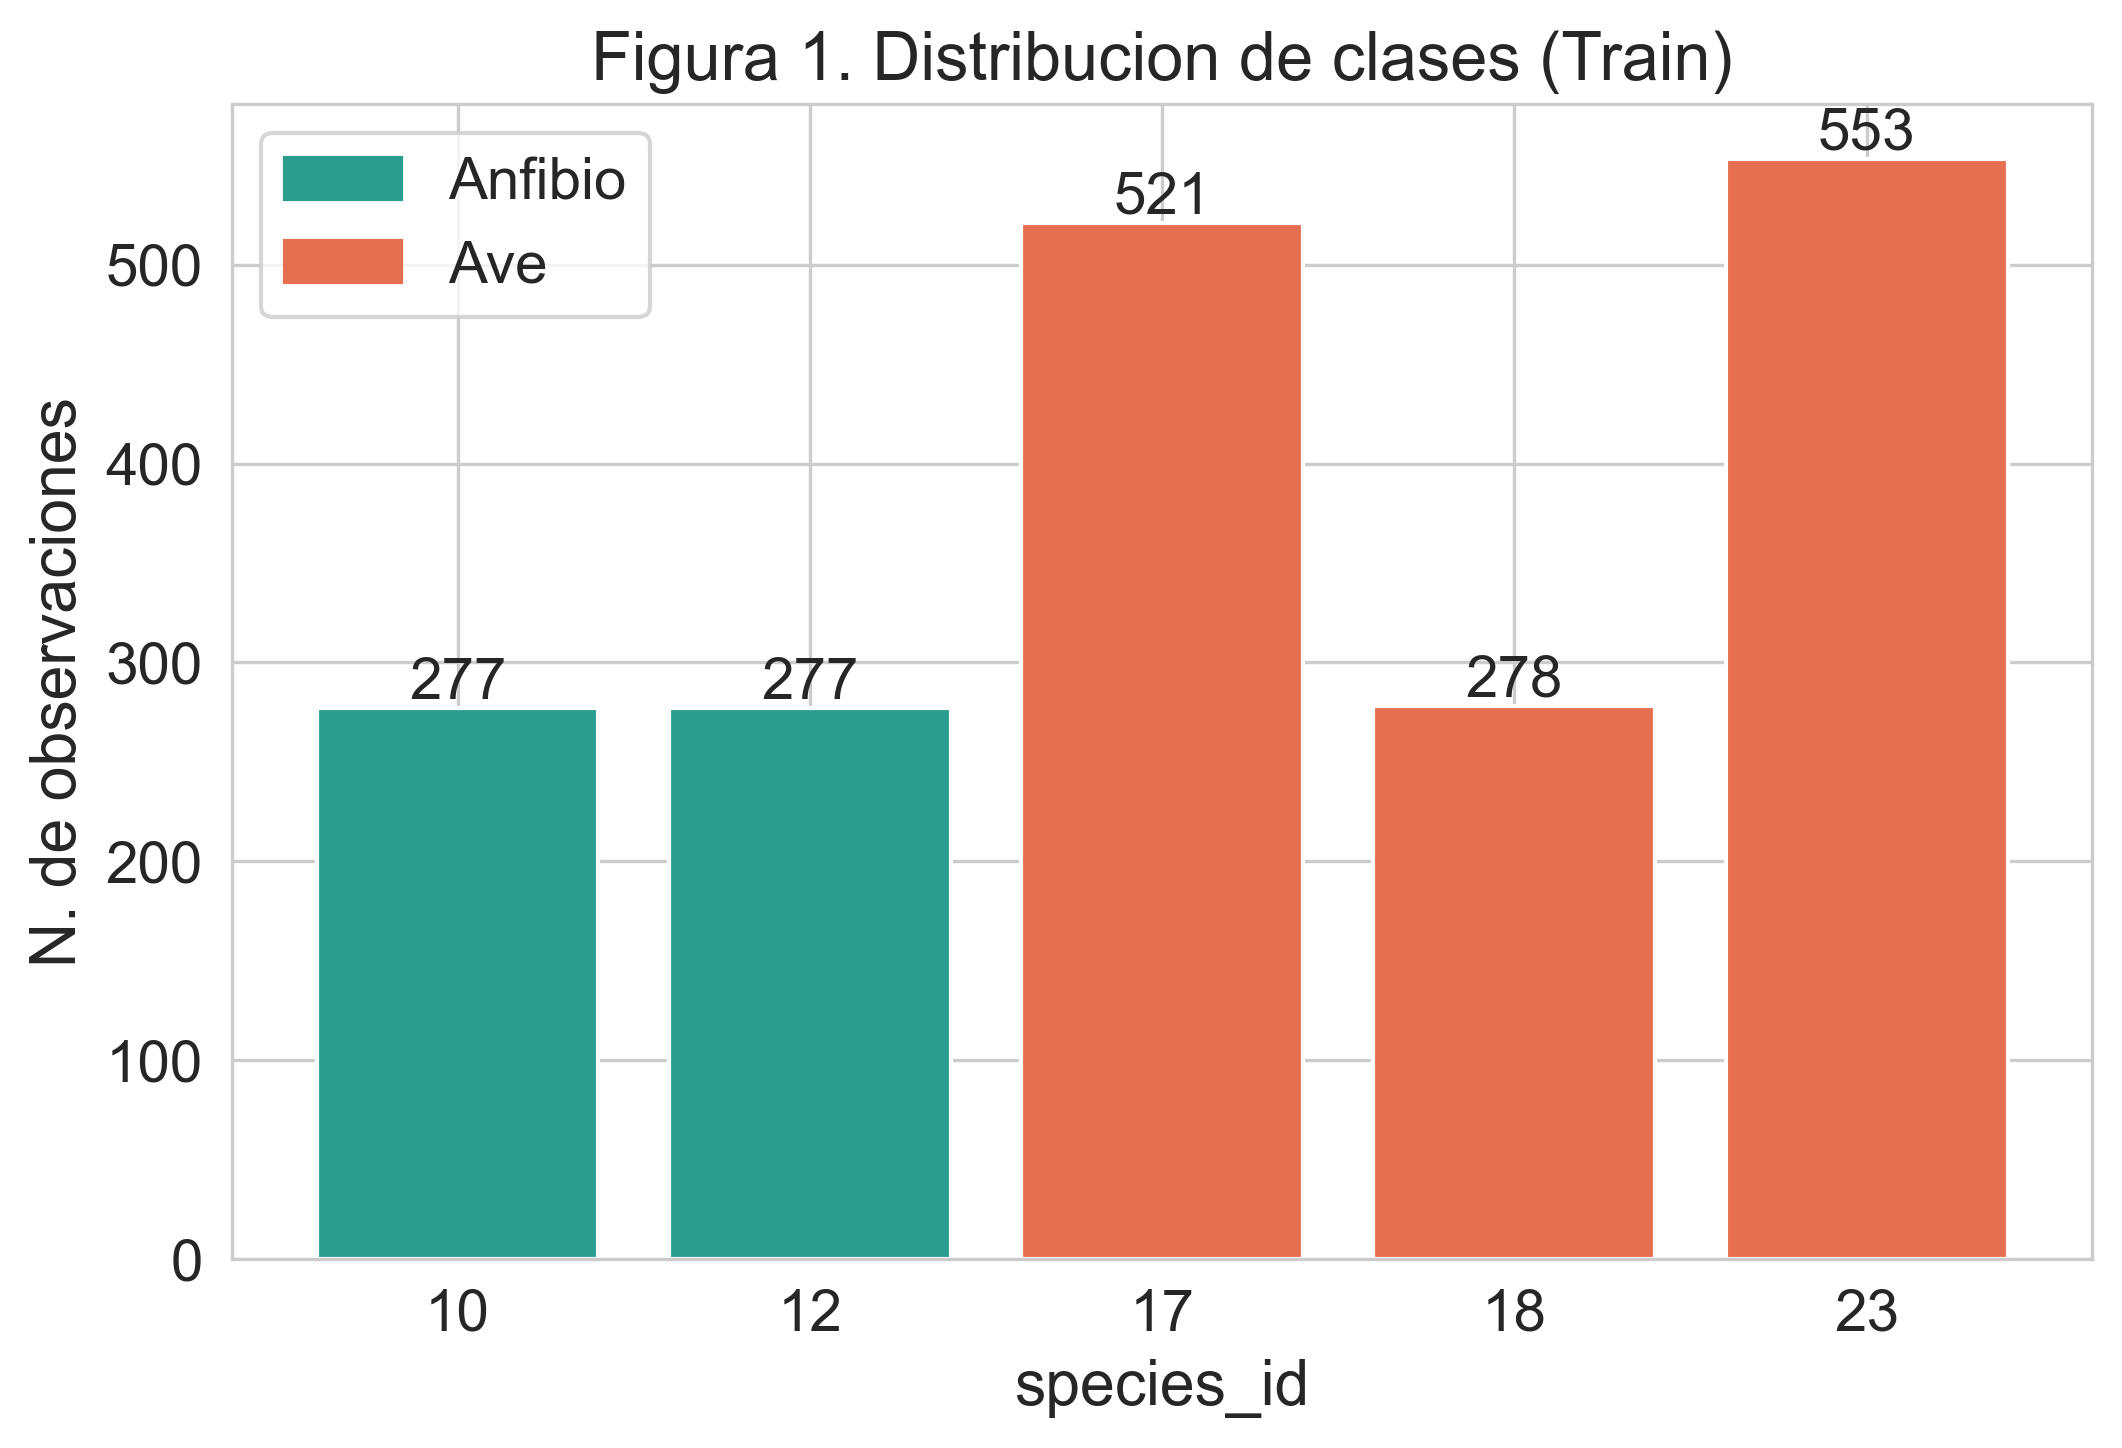
\includegraphics[width=0.55\textwidth]{figs/fig1_distribucion.png}
\caption{Distribuci\'on de clases en el conjunto de entrenamiento. Se evidencia el
desbalance entre especies, dominado por las clases 17 y 23.}
\label{fig:dist}
\end{figure}

\subsection{Arquitectura del pipeline}
La soluci\'on propuesta se estructura como un pipeline integral que abarca desde
la ingesta de los archivos CSV hasta la inferencia con mitigaci\'on de riesgos.
La Figura~\ref{fig:arq} ilustra el flujo completo: ingesta y separaci\'on de
predictoras/metadatos, estandarizaci\'on, exploraci\'on geom\'etrica mediante
reducci\'on de dimensionalidad, miner\'ia de patrones por clustering,
entrenamiento comparativo de clasificadores y, finalmente, la pol\'itica de
moderaci\'on basada en umbrales probabil\'isticos.

\begin{figure}[H]
\centering
\includegraphics[width=0.9\textwidth]{figs/fig_arquitectura.png}
\caption{Arquitectura del pipeline propuesto, desde la matriz base de
caracter\'isticas Mel hasta el despliegue informativo.}
\label{fig:arq}
\end{figure}

% ===================================================================
\section{Exploraci\'on Geom\'etrica y Reducci\'on de Dimensionalidad}
\label{sec:dr}
% ===================================================================

Con el objetivo de visualizar la estructura geom\'etrica del espacio
$\mathbb{R}^{64}$ y evaluar la separabilidad de las clases, se contrastaron un
m\'etodo lineal y dos m\'etodos de aproximaci\'on de variedades m\'ultiples.

\subsection{An\'alisis comparativo}
El \textbf{An\'alisis de Componentes Principales (PCA)} proyecta los datos sobre
los ejes ortogonales de m\'axima varianza, preservando la \textbf{estructura
global} de forma lineal. Se determin\'o que se requieren 7 componentes para
retener el 90\,\% de la varianza y 11 para el 95\,\%
(Figura~\ref{fig:pcavar}); las dos primeras componentes retienen \'unicamente
el 67{,}1\,\% de la varianza total, lo que anticipa un solapamiento al proyectar a 2D.

En contraste, \textbf{t-SNE} y \textbf{UMAP} son t\'ecnicas no lineales que
preservan las \textbf{distancias geom\'etricas locales}, priorizando que las
vecindades del espacio original se mantengan en la proyecci\'on de baja dimensi\'on.
La Figura~\ref{fig:proy2d} contrasta las tres proyecciones en 2D y la
Figura~\ref{fig:umap3d} muestra la proyecci\'on UMAP en 3D.

\begin{figure}[H]
\centering
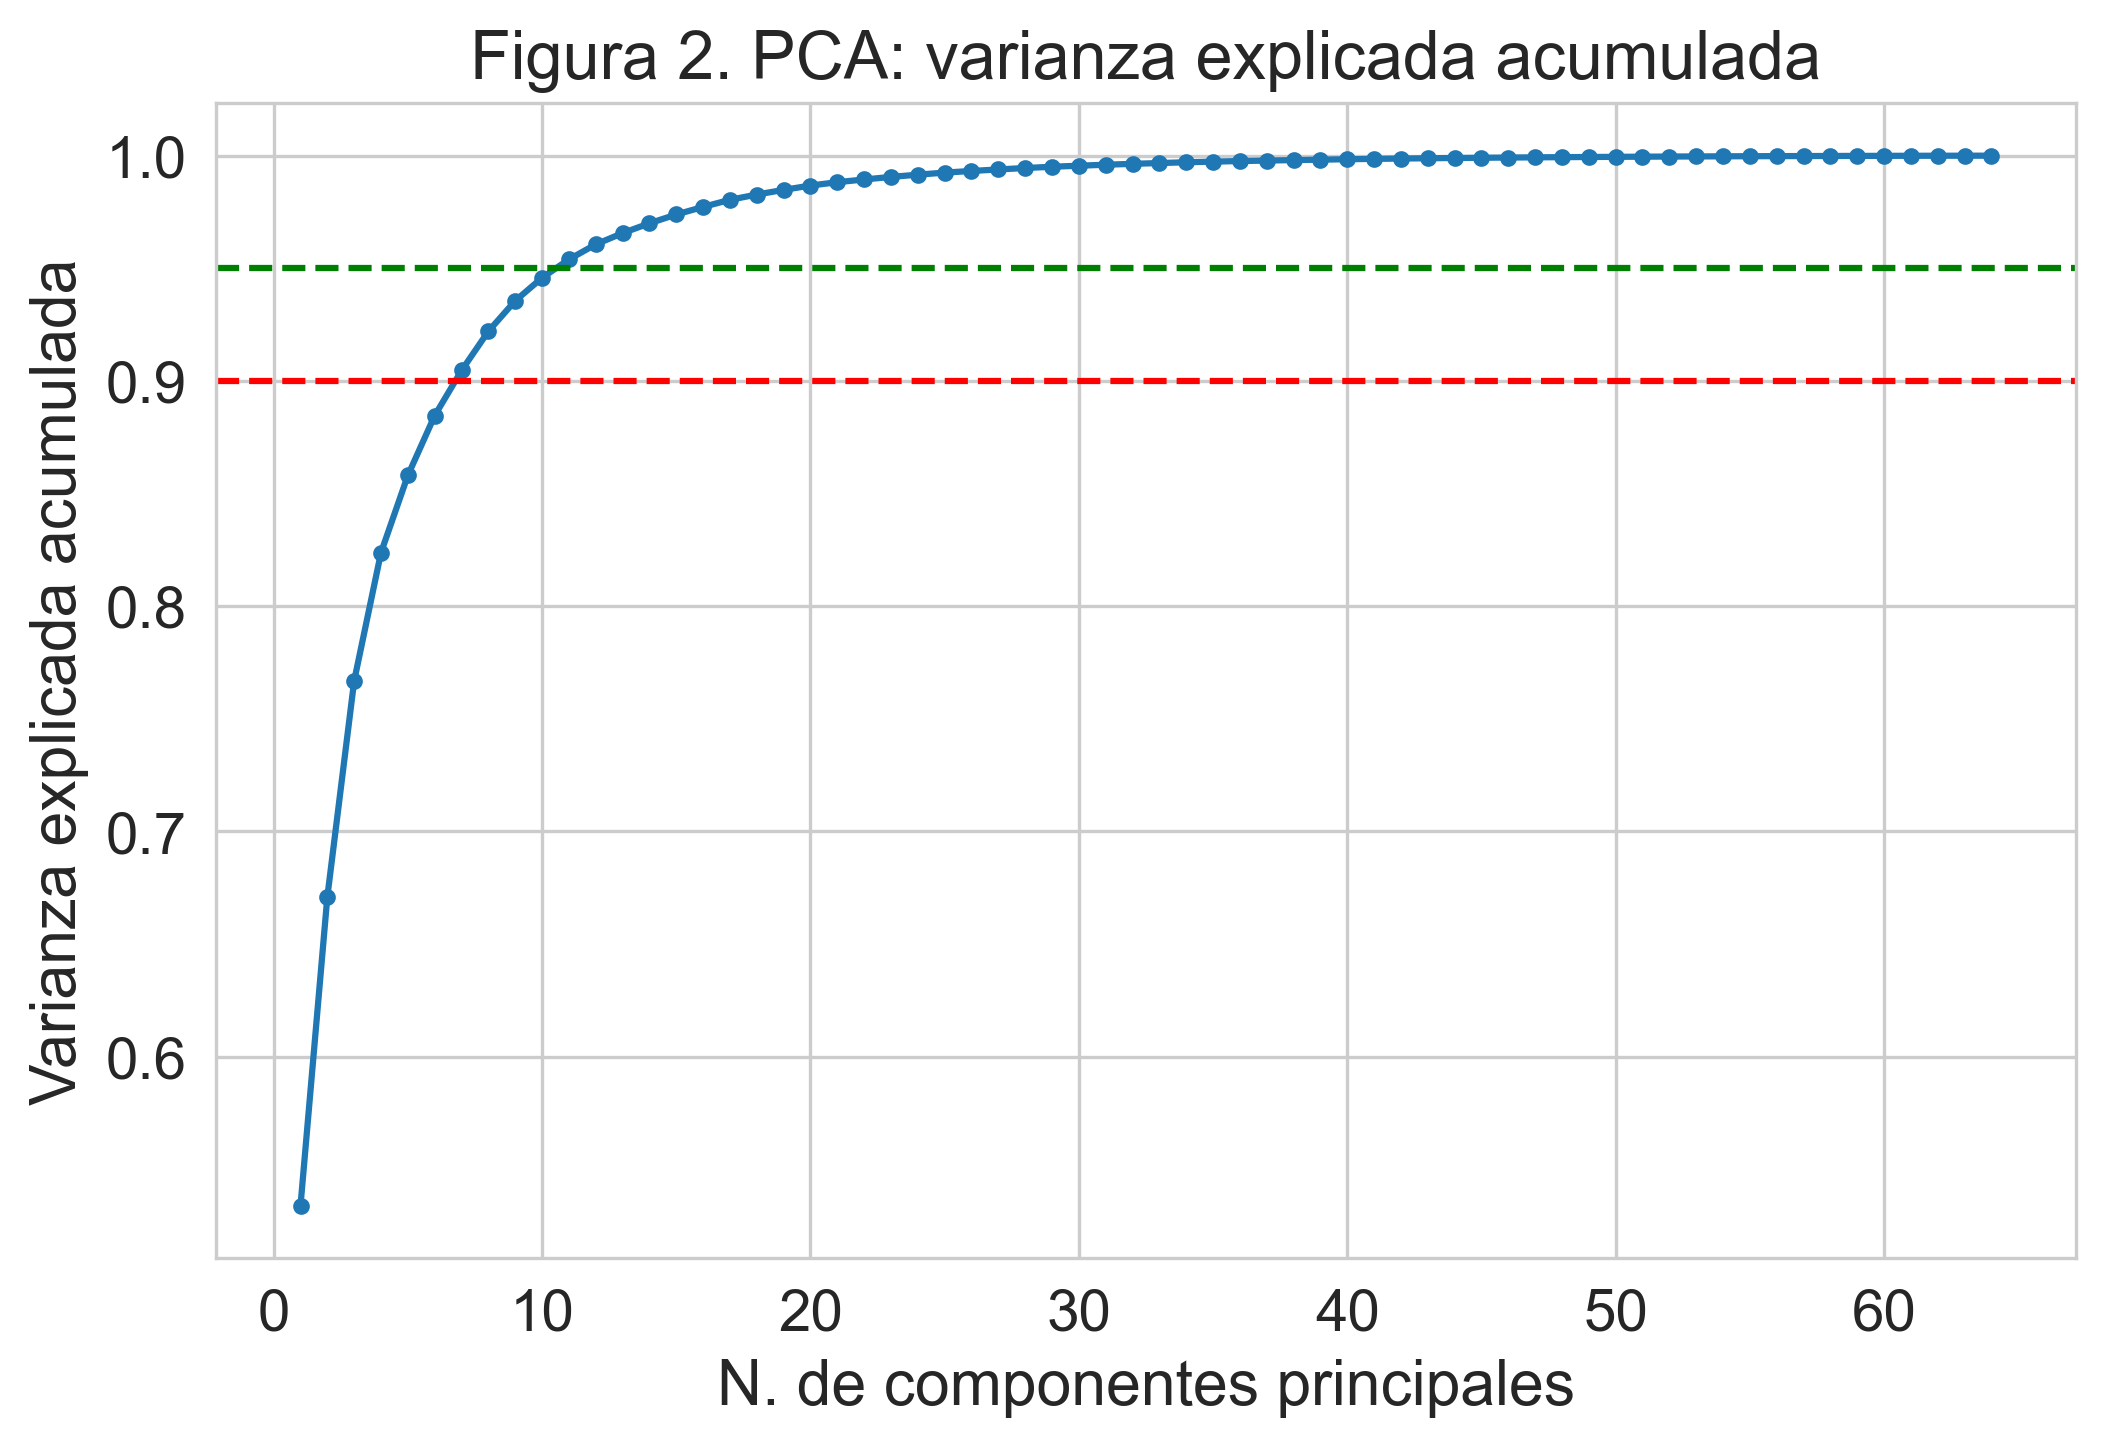
\includegraphics[width=0.55\textwidth]{figs/fig2_pca_varianza.png}
\caption{Varianza explicada acumulada en funci\'on del n\'umero de componentes
principales. Las l\'ineas punteadas indican los umbrales del 90\,\% y 95\,\%.}
\label{fig:pcavar}
\end{figure}

\begin{figure}[H]
\centering
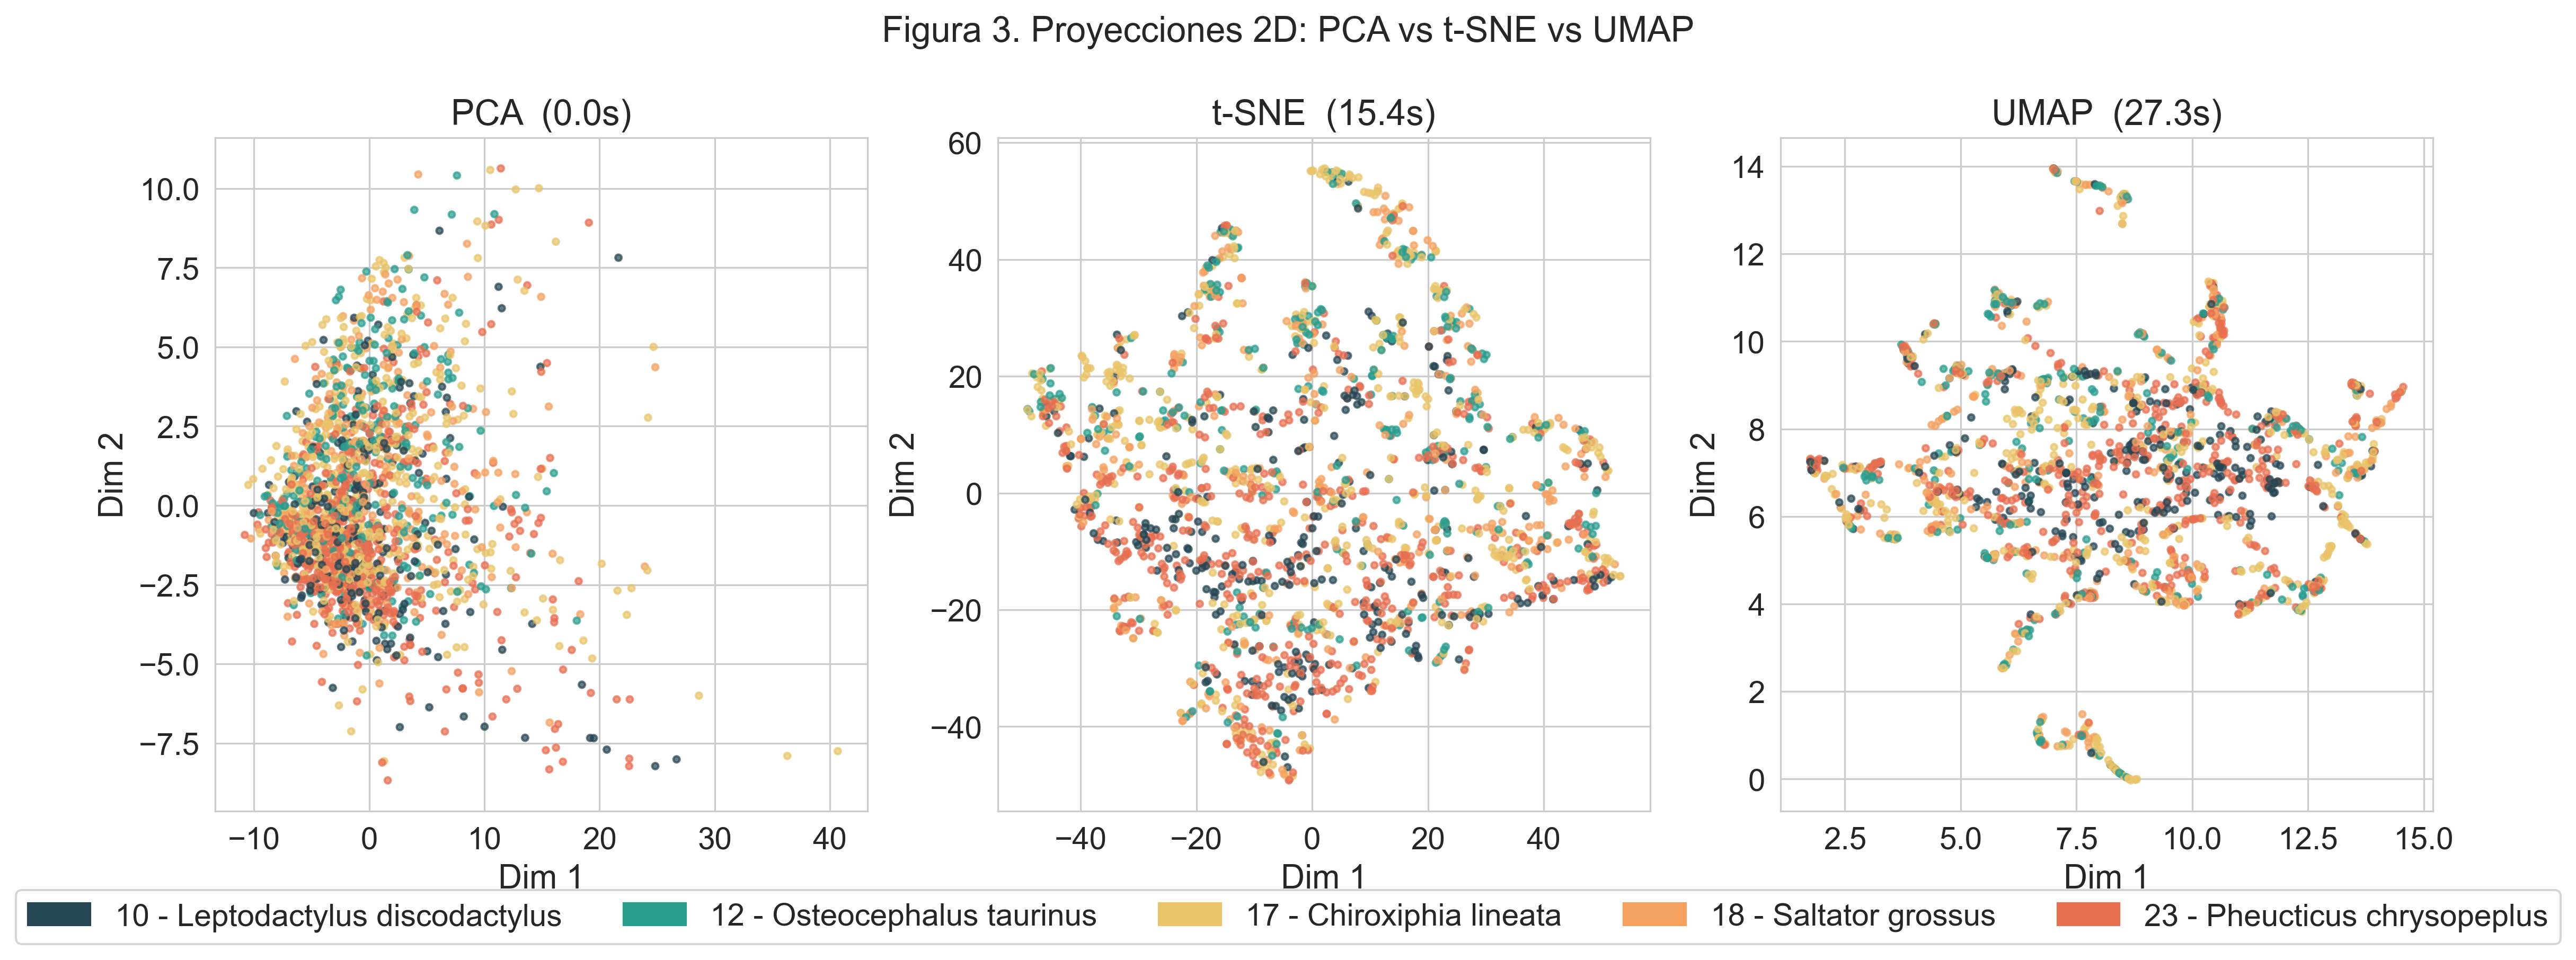
\includegraphics[width=0.95\textwidth]{figs/fig3_proyecciones2d.png}
\caption{Proyecciones 2D del espacio Mel coloreadas por especie: PCA (lineal)
frente a t-SNE y UMAP (variedades). Las t\'ecnicas no lineales separan mejor los
grupos que la proyecci\'on lineal.}
\label{fig:proy2d}
\end{figure}

\begin{figure}[H]
\centering
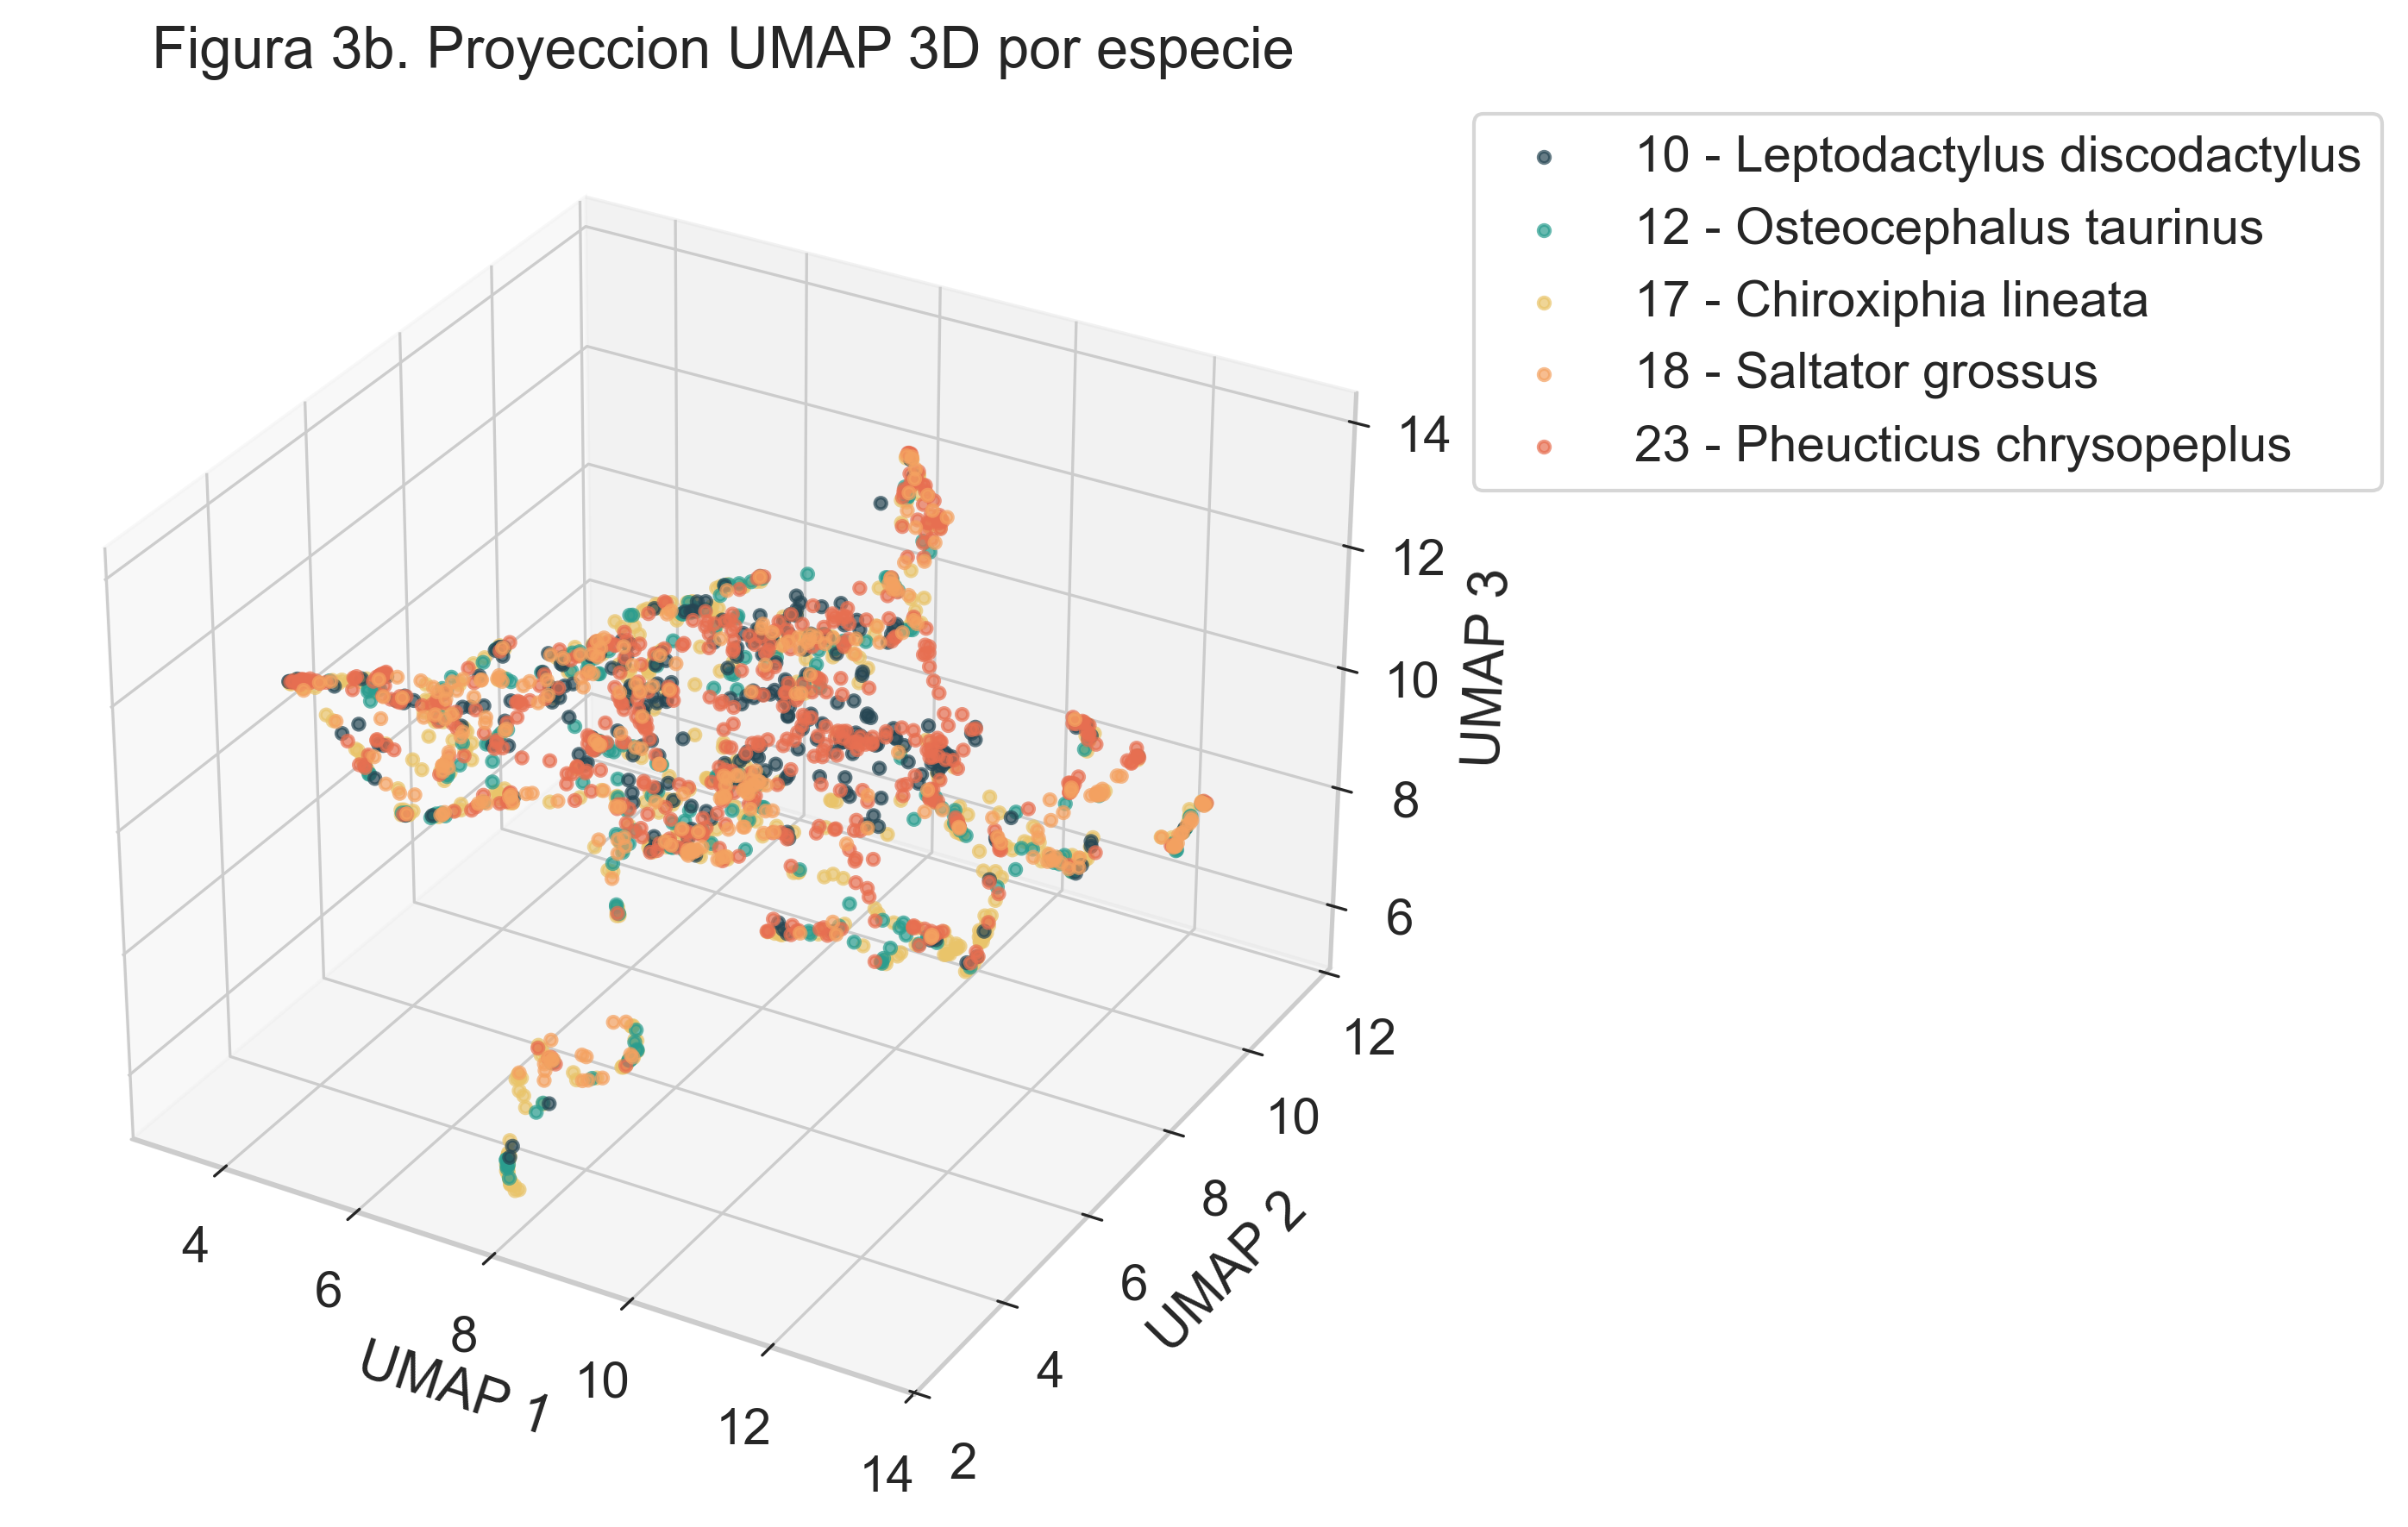
\includegraphics[width=0.6\textwidth]{figs/fig3b_umap3d.png}
\caption{Proyecci\'on UMAP en 3 dimensiones del conjunto de entrenamiento.}
\label{fig:umap3d}
\end{figure}

\subsection{Justificaci\'on t\'ecnica}
El Cuadro~\ref{tab:dr} reporta el compromiso entre costo computacional y retenci\'on
de estructura. PCA result\'o el m\'etodo m\'as eficiente ($0{,}01$\,s) por su naturaleza
algebraica, pero su \textit{trustworthiness} fue la menor, coherente con su
incapacidad de capturar relaciones no lineales. t-SNE y UMAP incrementaron el
tiempo de c\'omputo a $11{,}9$\,s y $11{,}3$\,s respectivamente, a cambio de una mayor
preservaci\'on de la estructura local (\textit{trustworthiness} de $0{,}987$ y $0{,}977$,
frente a $0{,}867$ de PCA). En
consecuencia, las t\'ecnicas de variedades resultan preferibles para la
\textbf{visualizaci\'on} y la inspecci\'on de separabilidad, mientras que PCA se
reserva como paso de \textbf{compresi\'on} previo al clustering por su bajo costo y
su interpretabilidad en t\'erminos de varianza.

\begin{table}[H]
\centering
\caption{Comparativa de m\'etodos de reducci\'on de dimensionalidad: tiempo de
ejecuci\'on y retenci\'on de estructura local (\textit{trustworthiness},
$k=10$).}
\label{tab:dr}
\small
\begin{tabular}{lccl}
\toprule
M\'etodo & Tiempo (s) & \textit{Trustworthiness} & Tipo \\
\midrule
PCA   & $0{,}01$  & $0{,}867$ & Lineal (varianza global) \\
t-SNE & $11{,}91$ & $0{,}987$ & Variedad (estructura local) \\
UMAP  & $11{,}26$ & $0{,}977$ & Variedad (estructura local) \\
\bottomrule
\end{tabular}
\end{table}

% ===================================================================
\section{Miner\'ia de Patrones y Estructuras de Clustering}
% ===================================================================

Se evaluaron dos algoritmos de aprendizaje no supervisado basados en paradigmas
distintos. Dado que, seg\'un la Secci\'on~\ref{sec:dr} (Figura~\ref{fig:pcavar}), $11$
componentes principales son suficientes para retener el $95\,\%$ de la varianza, el
clustering se aplic\'o sobre dicho subespacio en lugar del espacio original
$\mathbb{R}^{64}$. Esta compresi\'on previa reduce el ruido y el costo computacional
sin sacrificar informaci\'on relevante, y mitiga el efecto de la \textit{maldici\'on de
la dimensionalidad} sobre las m\'etricas basadas en distancias.

\subsection{Segmentaci\'on org\'anica}
El \textbf{Gaussian Mixture Model (GMM)} adopta un paradigma \textbf{probabil\'istico}:
modela los datos como una mezcla de $k$ distribuciones gaussianas y asigna a cada
punto una probabilidad de pertenencia (\textit{soft assignment}). El
\textbf{DBSCAN} adopta un paradigma de \textbf{densidad}: agrupa regiones densas y
etiqueta como ruido los puntos aislados, sin requerir la especificaci\'on previa
del n\'umero de grupos, pero con fuerte dependencia del hiperpar\'ametro $\varepsilon$.
El valor de $\varepsilon$ se estim\'o mediante el gr\'afico de $k$-distancia
(Figura~\ref{fig:kdist}), identificando el codo de la curva, y se realiz\'o un
barrido fino alrededor de dicho valor.

\subsection{M\'etricas de validaci\'on}
La elecci\'on del n\'umero \'optimo de grupos se sustent\'o exclusivamente en
\textbf{m\'etricas internas} (que no emplean las etiquetas reales): el
\textbf{Coeficiente de Silhouette}, el \'indice de \textbf{Davies-Bouldin} y el de
\textbf{Calinski-Harabasz} (Figura~\ref{fig:metricas}). El criterio de Silhouette
sugiri\'o $k=2$ grupos para GMM ($s=0{,}184$), valor corroborado por las restantes
m\'etricas internas (m\'inimo de Davies-Bouldin y m\'aximo de Calinski-Harabasz en $k=2$)
y por el criterio BIC (Figura~\ref{fig:gmmsel}). El Cuadro~
\ref{tab:clust} sintetiza el desempe\~no; adicionalmente, el \'indice de Rand
ajustado (ARI), calculado de forma externa, cuantifica el grado de alineaci\'on
entre los grupos descubiertos y la taxonom\'ia real.

\begin{figure}[H]
\centering
\begin{subfigure}{0.48\textwidth}
  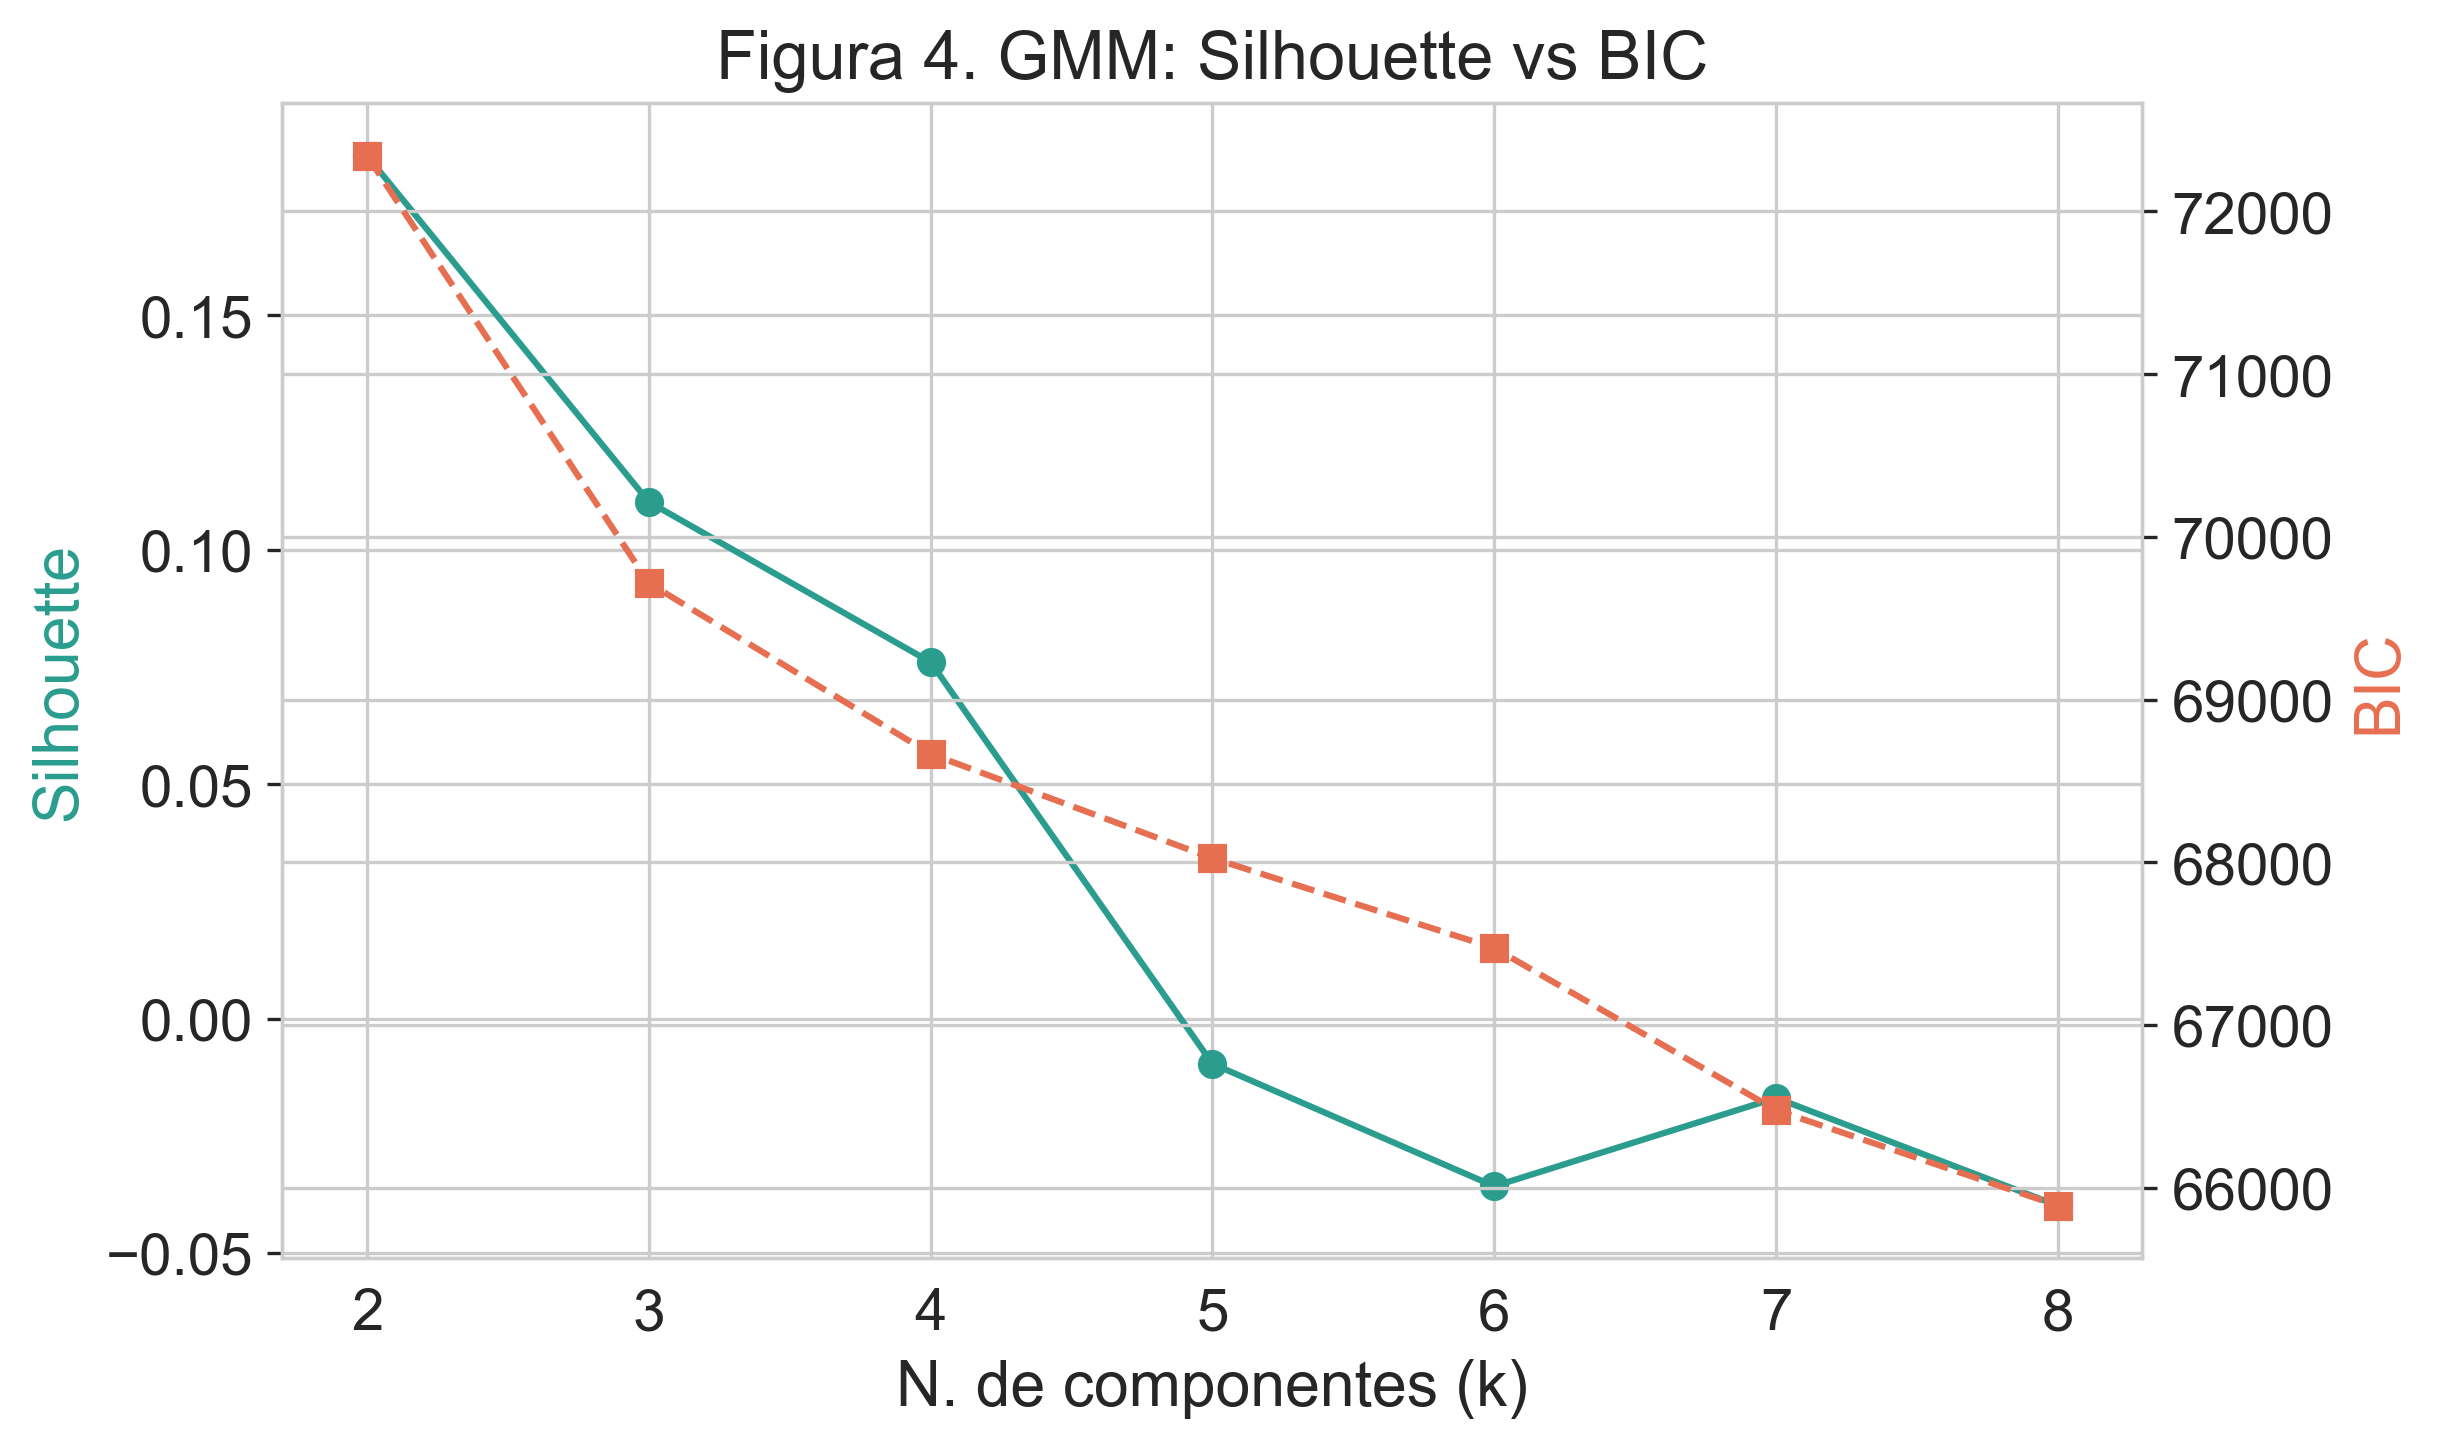
\includegraphics[width=\textwidth]{figs/fig4_gmm_silhouette_bic.png}
  \caption{GMM: Silhouette y BIC frente a $k$.}
  \label{fig:gmmsel}
\end{subfigure}\hfill
\begin{subfigure}{0.48\textwidth}
  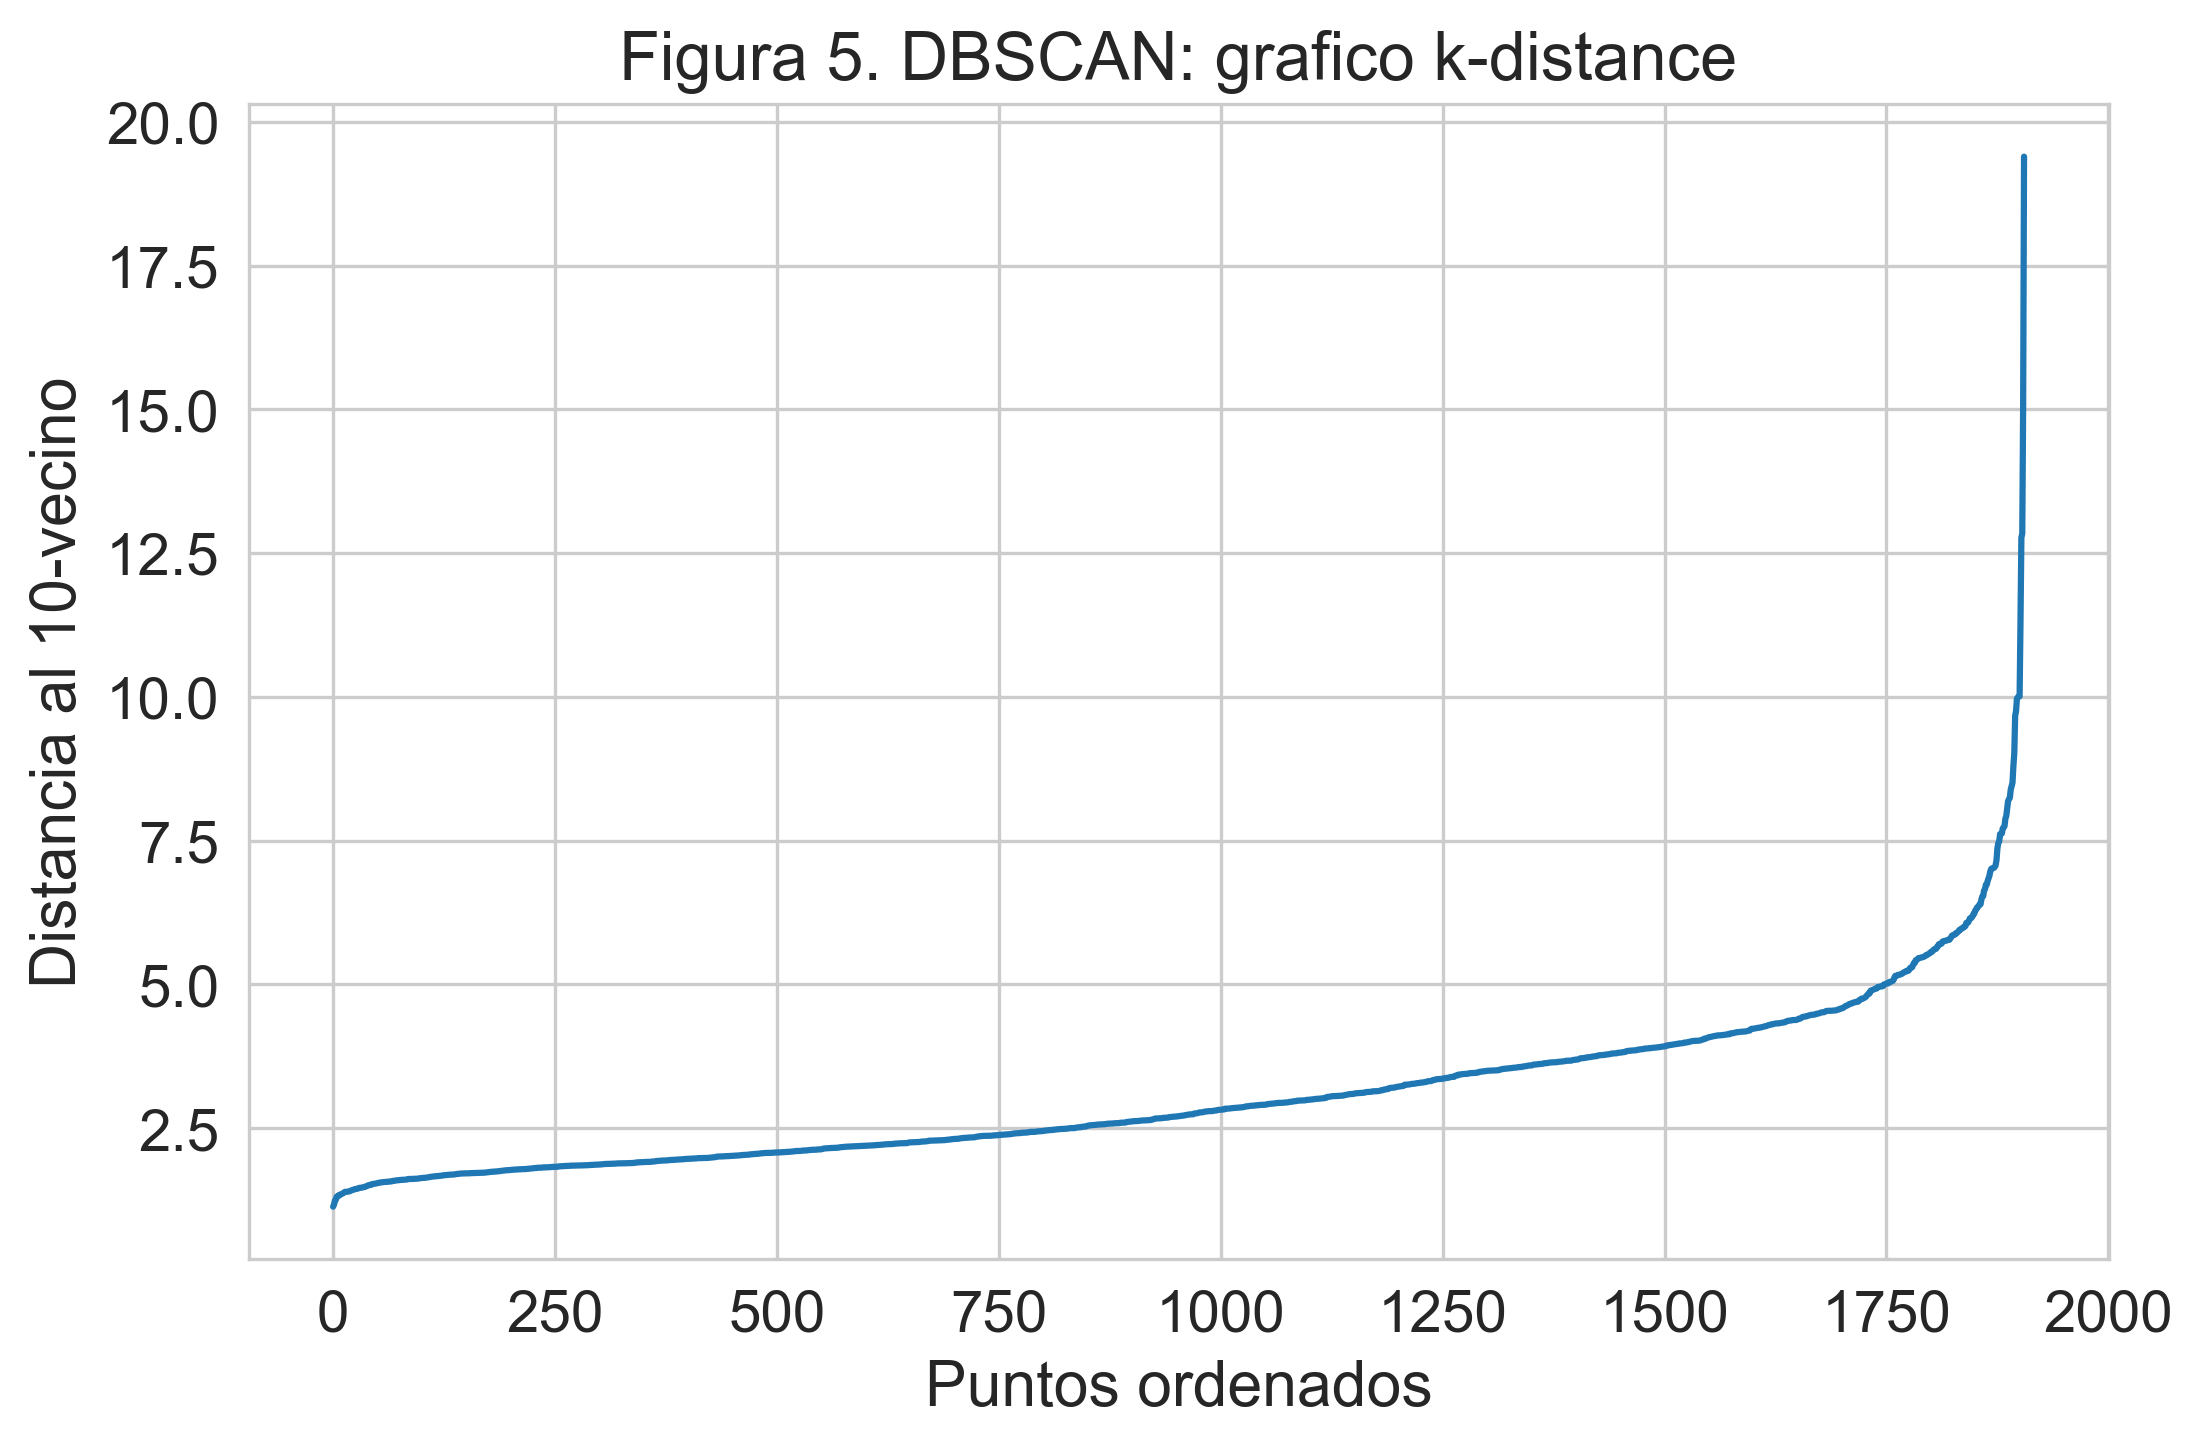
\includegraphics[width=\textwidth]{figs/fig5_dbscan_kdist.png}
  \caption{DBSCAN: gr\'afico de $k$-distancia.}
  \label{fig:kdist}
\end{subfigure}
\caption{Selecci\'on de hiperpar\'ametros para los dos algoritmos de clustering.}
\end{figure}

\begin{figure}[H]
\centering
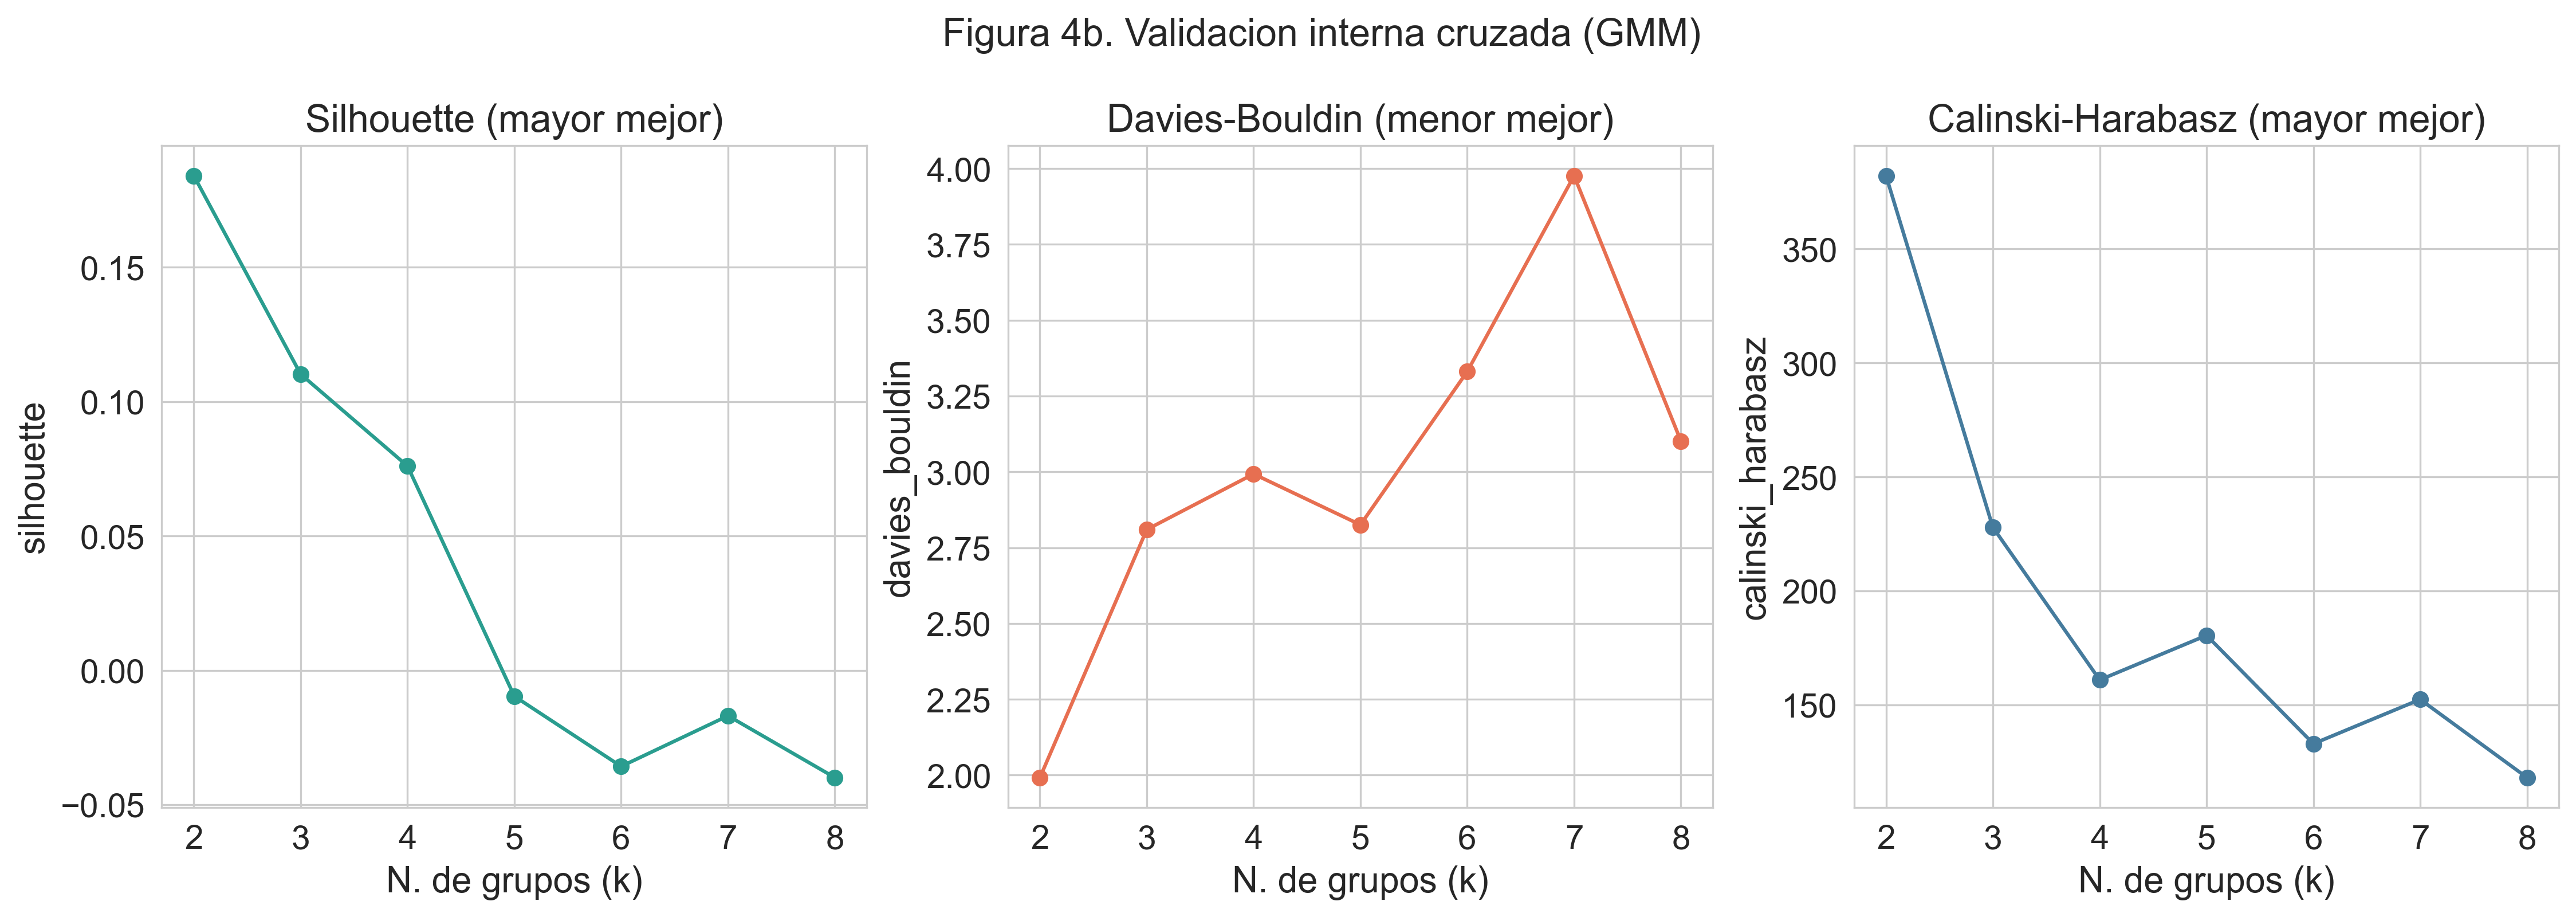
\includegraphics[width=0.95\textwidth]{figs/fig4b_metricas_internas.png}
\caption{Validaci\'on interna cruzada del n\'umero de grupos en GMM mediante
Silhouette, Davies-Bouldin y Calinski-Harabasz.}
\label{fig:metricas}
\end{figure}

\begin{table}[H]
\centering
\caption{Comparativa de los algoritmos de clustering. ARI se reporta como
referencia externa de alineaci\'on con \texttt{species\_id}.}
\label{tab:clust}
\small
\begin{tabular}{lcccc}
\toprule
M\'etodo & Paradigma & Grupos & Silhouette & ARI \\
\midrule
GMM    & Probabil\'istico & 2 & $0{,}184$ & $0{,}026$ \\
DBSCAN & Densidad        & 2 & --       & $0{,}004$ \\
\bottomrule
\end{tabular}
\end{table}

Los valores de Silhouette pr\'oximos a cero y los \'indices ARI cercanos a $0$
($0{,}026$ para GMM y $0{,}004$ para DBSCAN) constituyen un hallazgo relevante: la
estructura no supervisada del espacio Mel \textbf{no se organiza en cinco grupos
densos separables} que coincidan con la taxonom\'ia. Ambos algoritmos favorecen
$k=2$, lo que sugiere una separaci\'on macrosc\'opica (posiblemente se\~nal robusta
frente a registros ruidosos, o anfibios frente a aves) antes que la discriminaci\'on
fina entre especies. Este solapamiento ac\'ustico anticipa la dificultad intr\'inseca
de la tarea de clasificaci\'on supervisada abordada en la siguiente secci\'on.

% ===================================================================
\section{Arquitectura de Clasificaci\'on: MLP vs. Modelos de Ensamble}
% ===================================================================

\subsection{Dise\~no de la red neuronal}
Se implement\'o un Perceptr\'on Multicapa (MLP) en PyTorch. Para la clasificaci\'on
multiclase se emple\'o como funci\'on de p\'erdida la \textbf{entrop\'ia cruzada
categ\'orica ponderada}. Dada una observaci\'on con logits de salida
$\mathbf{z} = (z_1, \dots, z_C)$, la capa \textit{softmax} produce la distribuci\'on
de probabilidad
\begin{equation}
\hat{p}_k = \frac{e^{z_k}}{\sum_{j=1}^{C} e^{z_j}}, \qquad k = 1,\dots,C,
\end{equation}
y la p\'erdida total sobre $N$ observaciones se define como
\begin{equation}
\mathcal{L} = -\sum_{i=1}^{N} w_{y_i} \, \log \hat{p}_{i,\,y_i},
\end{equation}
donde $y_i$ es la clase verdadera de la muestra $i$ y $w_{y_i}$ es el peso asignado
a dicha clase, calculado de forma inversamente proporcional a su frecuencia para
\textbf{compensar el desbalance}. El Cuadro~\ref{tab:topo} detalla la topolog\'ia de
la red.

\begin{table}[H]
\centering
\caption{Topolog\'ia de la red MLP (configuraci\'on recomendada
Linear$\to$BatchNorm$\to$ReLU$\to$Dropout).}
\label{tab:topo}
\small
\begin{tabular}{clcc}
\toprule
Capa & Tipo & Neuronas & Activaci\'on \\
\midrule
Entrada & --              & 64  & --   \\
Oculta 1 & Linear+BN+Dropout & 128 & ReLU \\
Oculta 2 & Linear+BN+Dropout & 64  & ReLU \\
Salida   & Linear            & 5   & Softmax \\
\bottomrule
\end{tabular}
\end{table}

\subsection{Estrategia de regularizaci\'on}
Se analiz\'o emp\'iricamente el impacto de la \textbf{posici\'on relativa} de las
capas de Dropout y Batch Normalization sobre la estabilidad de las curvas de
aprendizaje. La Figura~\ref{fig:curvas} contrasta el orden
Linear$\to$BatchNorm$\to$ReLU$\to$Dropout frente a
Linear$\to$Dropout$\to$BatchNorm$\to$ReLU. Se observ\'o que la configuraci\'on
Linear$\to$BatchNorm$\to$ReLU$\to$Dropout produjo curvas de validaci\'on m\'as
estables y una menor brecha entre las p\'erdidas de entrenamiento y validaci\'on,
raz\'on por la cual fue adoptada en el modelo final. Situar la normalizaci\'on antes
del \textit{dropout} permite que las estad\'isticas de cada \textit{batch} se estimen
sobre activaciones completas, evitando la inestabilidad que introduce normalizar
sobre un subconjunto ya diezmado de neuronas. No obstante, en ambas configuraciones
se observa que, a partir de la \'epoca $\sim\!20$, la p\'erdida de validaci\'on se
estabiliza e incluso repunta ligeramente mientras la de entrenamiento contin\'ua
descendiendo: una se\~nal de \textbf{sobreajuste leve} que la regularizaci\'on acota
pero no elimina. Este comportamiento justifica el uso de \textit{dropout} y sugiere que
la incorporaci\'on de \textit{early stopping} en torno a dicha \'epoca constituir\'ia una
mejora directa para futuras iteraciones.

\begin{figure}[H]
\centering
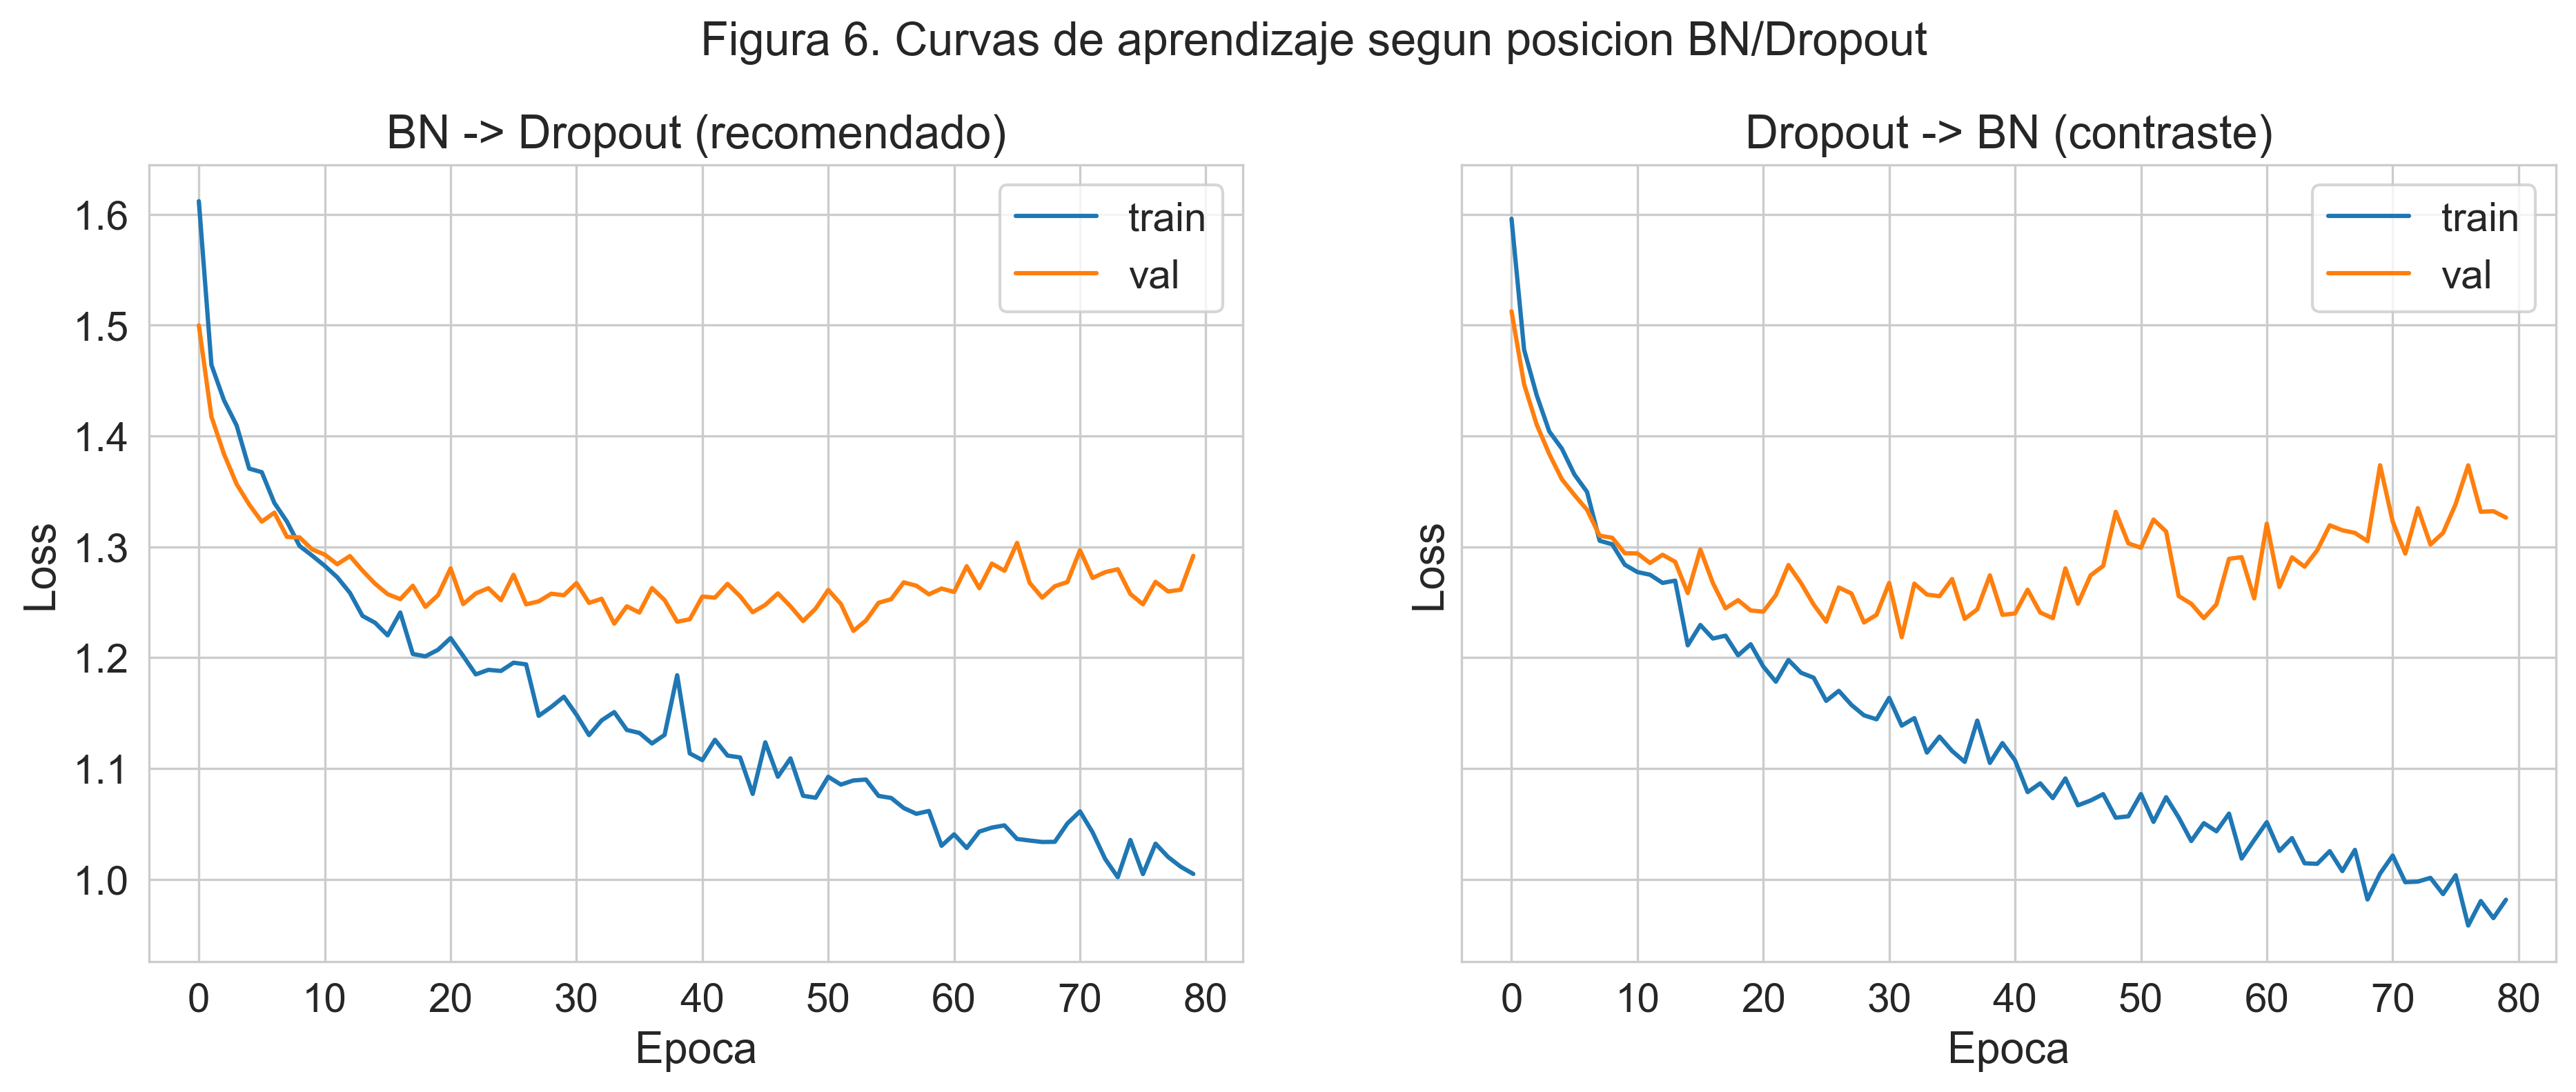
\includegraphics[width=0.95\textwidth]{figs/fig6_curvas_aprendizaje.png}
\caption{Curvas de aprendizaje (p\'erdida frente a \'epocas) seg\'un la posici\'on
relativa de las capas de Batch Normalization y Dropout.}
\label{fig:curvas}
\end{figure}

\subsection{Benchmarking computacional}
El MLP se compar\'o contra \textbf{XGBoost}, un modelo de ensamble basado en
\textit{gradient boosting} de \'arboles de decisi\'on. La evaluaci\'on se sostuvo
sobre el \textbf{F1-Score macro} y el an\'alisis de las \textbf{matrices de
confusi\'on} (Figura~\ref{fig:cm}), dada la inadecuaci\'on de la m\'etrica
\textit{accuracy} ante el desbalance de clases. El MLP alcanz\'o un F1-macro de
$0{,}453$, mientras que XGBoost obtuvo $0{,}466$, situando a ambos modelos
sensiblemente por encima del azar te\'orico ($\approx 0{,}20$ para cinco clases) pero
en un r\'egimen de dificultad elevada, coherente con el solapamiento detectado en la
fase no supervisada. El modelo de ensamble super\'o marginalmente a la red neuronal.
Un an\'alisis desagregado por clase (Cuadro~\ref{tab:recall}) matiza esta lectura.
El XGBoost concentra su acierto en las clases mayoritarias --recall de $0{,}66$ en la
clase 23 y $0{,}54$ en la 17--, a costa de penalizar severamente a las minoritarias
(recall de $0{,}34$ en la clase 12). El MLP, gracias a la ponderaci\'on de la
p\'erdida, distribuye el acierto de forma m\'as equitativa entre clases (recall de
$0{,}61$ en la clase 10 y $0{,}55$ en la 18), lo que explica que su F1-macro no se
distancie del ensamble pese a su menor \textit{accuracy} global. El error dominante no
se limita a las tres aves: la mayor masa de confusi\'on se produce entre las clases 23
(ave) y 10 (anfibio) en ambos modelos ($44$ casos $23\!\to\!10$ en el MLP y $29$ casos
$10\!\to\!23$ en XGBoost), lo que sugiere que el solapamiento en el espacio Mel
trasciende la frontera taxonom\'ica y refuerza la dificultad intr\'inseca anticipada por
el an\'alisis no supervisado.

\begin{table}[H]
\centering
\caption{Recall por clase en el conjunto de prueba. El MLP (con p\'erdida ponderada)
reparte el acierto de forma m\'as homog\'enea; XGBoost privilegia las clases
mayoritarias.}
\label{tab:recall}
\small
\begin{tabular}{cccccc}
\toprule
Modelo & Clase 10 & Clase 12 & Clase 17 & Clase 18 & Clase 23 \\
\midrule
MLP     & $0{,}61$ & $0{,}51$ & $0{,}41$ & $0{,}55$ & $0{,}33$ \\
XGBoost & $0{,}39$ & $0{,}34$ & $0{,}54$ & $0{,}36$ & $0{,}66$ \\
\bottomrule
\end{tabular}
\end{table}

\begin{figure}[H]
\centering
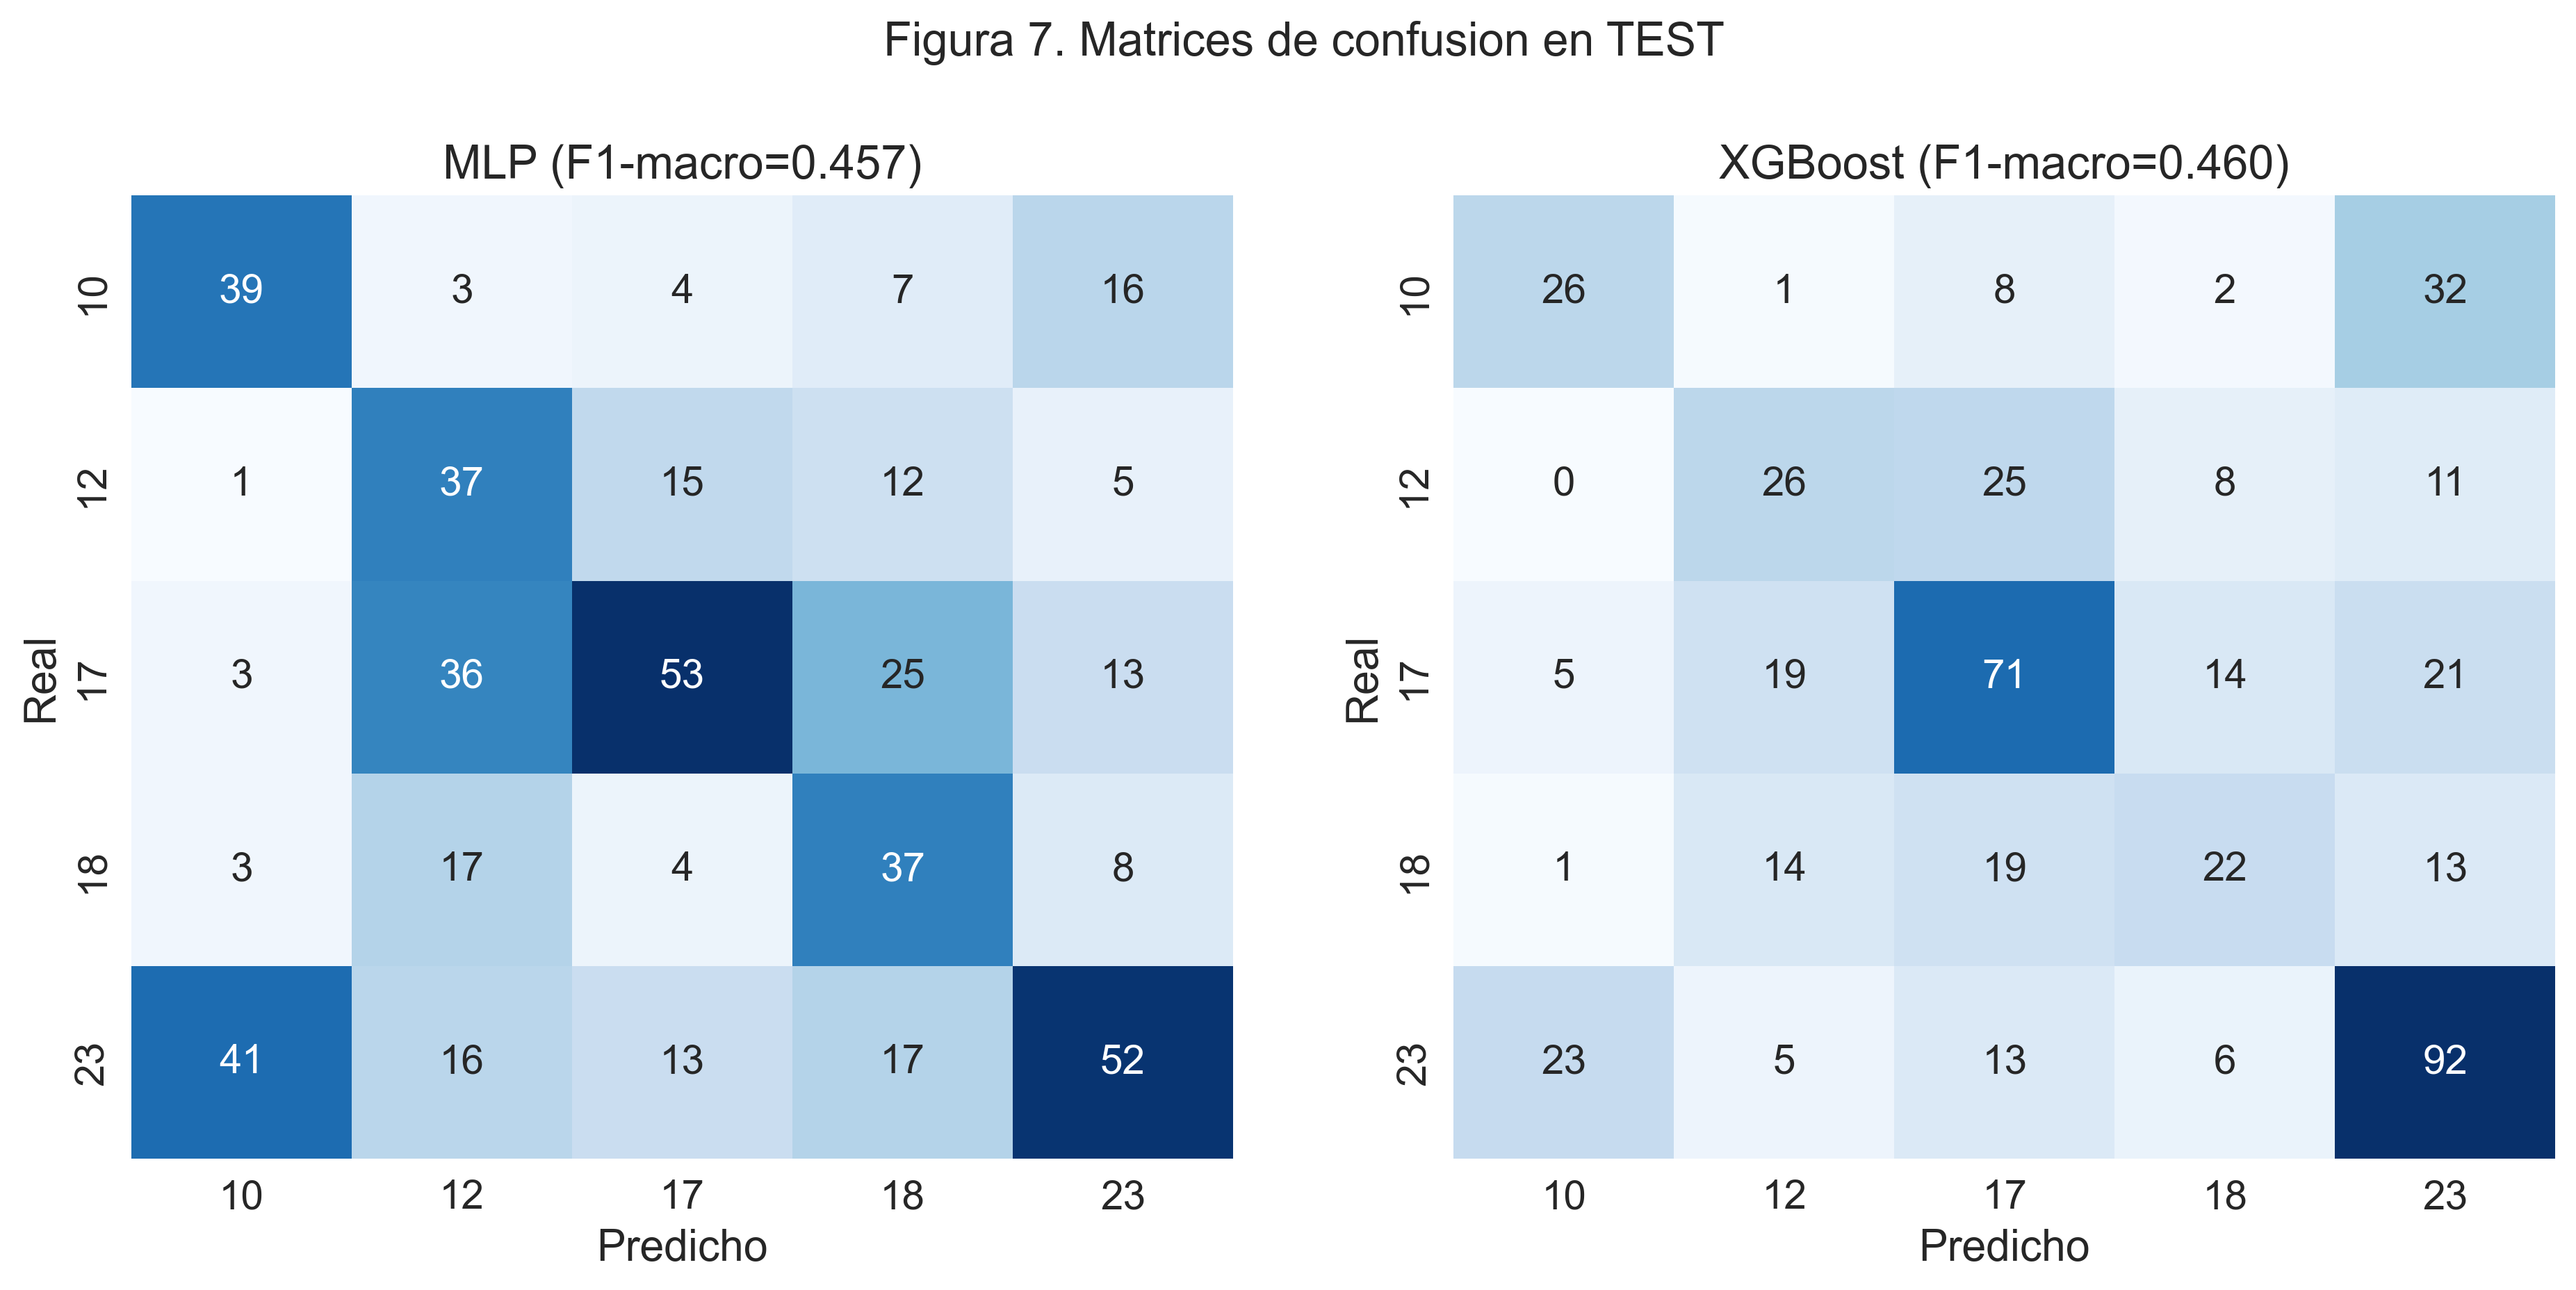
\includegraphics[width=0.95\textwidth]{figs/fig7_matrices_confusion.png}
\caption{Matrices de confusi\'on en el conjunto de prueba para el MLP (izquierda) y
XGBoost (derecha).}
\label{fig:cm}
\end{figure}

% ===================================================================
\section{Decisiones de Ingenier\'ia y Mitigaci\'on de Riesgos}
% ===================================================================

\subsection{An\'alisis de \textit{trade-offs}}
La selecci\'on del modelo de despliegue contempla el compromiso entre rendimiento
anal\'itico y costo computacional. El Cuadro~\ref{tab:tradeoff} contrasta el
F1-macro frente al tiempo de inferencia por registro. Si bien XGBoost
ofrece el mejor F1-macro ($0{,}466$), su tiempo de inferencia de $0{,}830$\,ms por
registro es aproximadamente $3{,}6$ veces superior al del MLP ($0{,}229$\,ms), lo que
debe ponderarse frente al volumen de registros esperado en producci\'on. Dada la
diferencia marginal en rendimiento, el MLP constituye una alternativa competitiva
cuando la latencia es cr\'itica.

\begin{table}[H]
\centering
\caption{Compromiso entre rendimiento (F1-macro) y costo (tiempo de inferencia por
registro).}
\label{tab:tradeoff}
\small
\begin{tabular}{lcc}
\toprule
Modelo & F1-macro & Inferencia (ms/registro) \\
\midrule
MLP     & $0{,}453$ & $0{,}229$ \\
XGBoost & $0{,}466$ & $0{,}830$ \\
\bottomrule
\end{tabular}
\end{table}

\subsection{Pol\'iticas de moderaci\'on}
Se dise\~n\'o una pol\'itica operativa basada en el vector de probabilidades de
salida del modelo \'optimo, que define tres estados seg\'un la probabilidad
predictiva m\'axima $P = \max_k \hat{p}_k$:
\begin{itemize}[noitemsep,topsep=2pt]
  \item \textbf{Zona de Confianza} ($P \geq 0.85$): clasificaci\'on autom\'atica
  (alerta verde). Cubri\'o el $19{,}9$\,\% de los registros de prueba (95 de 477),
  con una exactitud de $0{,}589$ en dicha zona.
  \item \textbf{Zona de Incertidumbre} ($0.40 \leq P < 0.85$): clasificaci\'on
  asistida; el registro se deriva a una cola de auditor\'ia humana (alerta amarilla).
  \item \textbf{Zona de Rechazo} ($P < 0.40$): descarte autom\'atico para mitigar el
  impacto del ruido ambiental (alerta roja).
\end{itemize}
La Figura~\ref{fig:zonas} muestra la distribuci\'on de la confianza del modelo y la
ubicaci\'on de los umbrales. Esta pol\'itica permite derivar la incertidumbre a
revisi\'on experta y controlar los falsos positivos. Cabe se\~nalar, sin embargo, una
limitaci\'on cr\'itica: la exactitud en la Zona de Confianza ($0{,}589$) es solo
moderadamente superior a la \textit{accuracy} global del modelo, lo que indica que una
probabilidad m\'axima $P\geq 0{,}85$ \textbf{no garantiza} una alta tasa de acierto. Ello
revela un modelo \textbf{insuficientemente calibrado}: las probabilidades de salida
sobreestiman la confianza real. En un despliegue productivo ser\'ia recomendable, o bien
elevar el umbral de automatizaci\'on, o bien aplicar una calibraci\'on posterior (p.\,ej.
\textit{temperature scaling} o regresi\'on isot\'onica) antes de confiar en la
clasificaci\'on autom\'atica. Dada la criticidad ecol\'ogica de un falso positivo, la
pol\'itica conservadora actual --que env\'ia el $75{,}7\,\%$ de los registros a auditoria--
resulta prudente.

\begin{figure}[H]
\centering
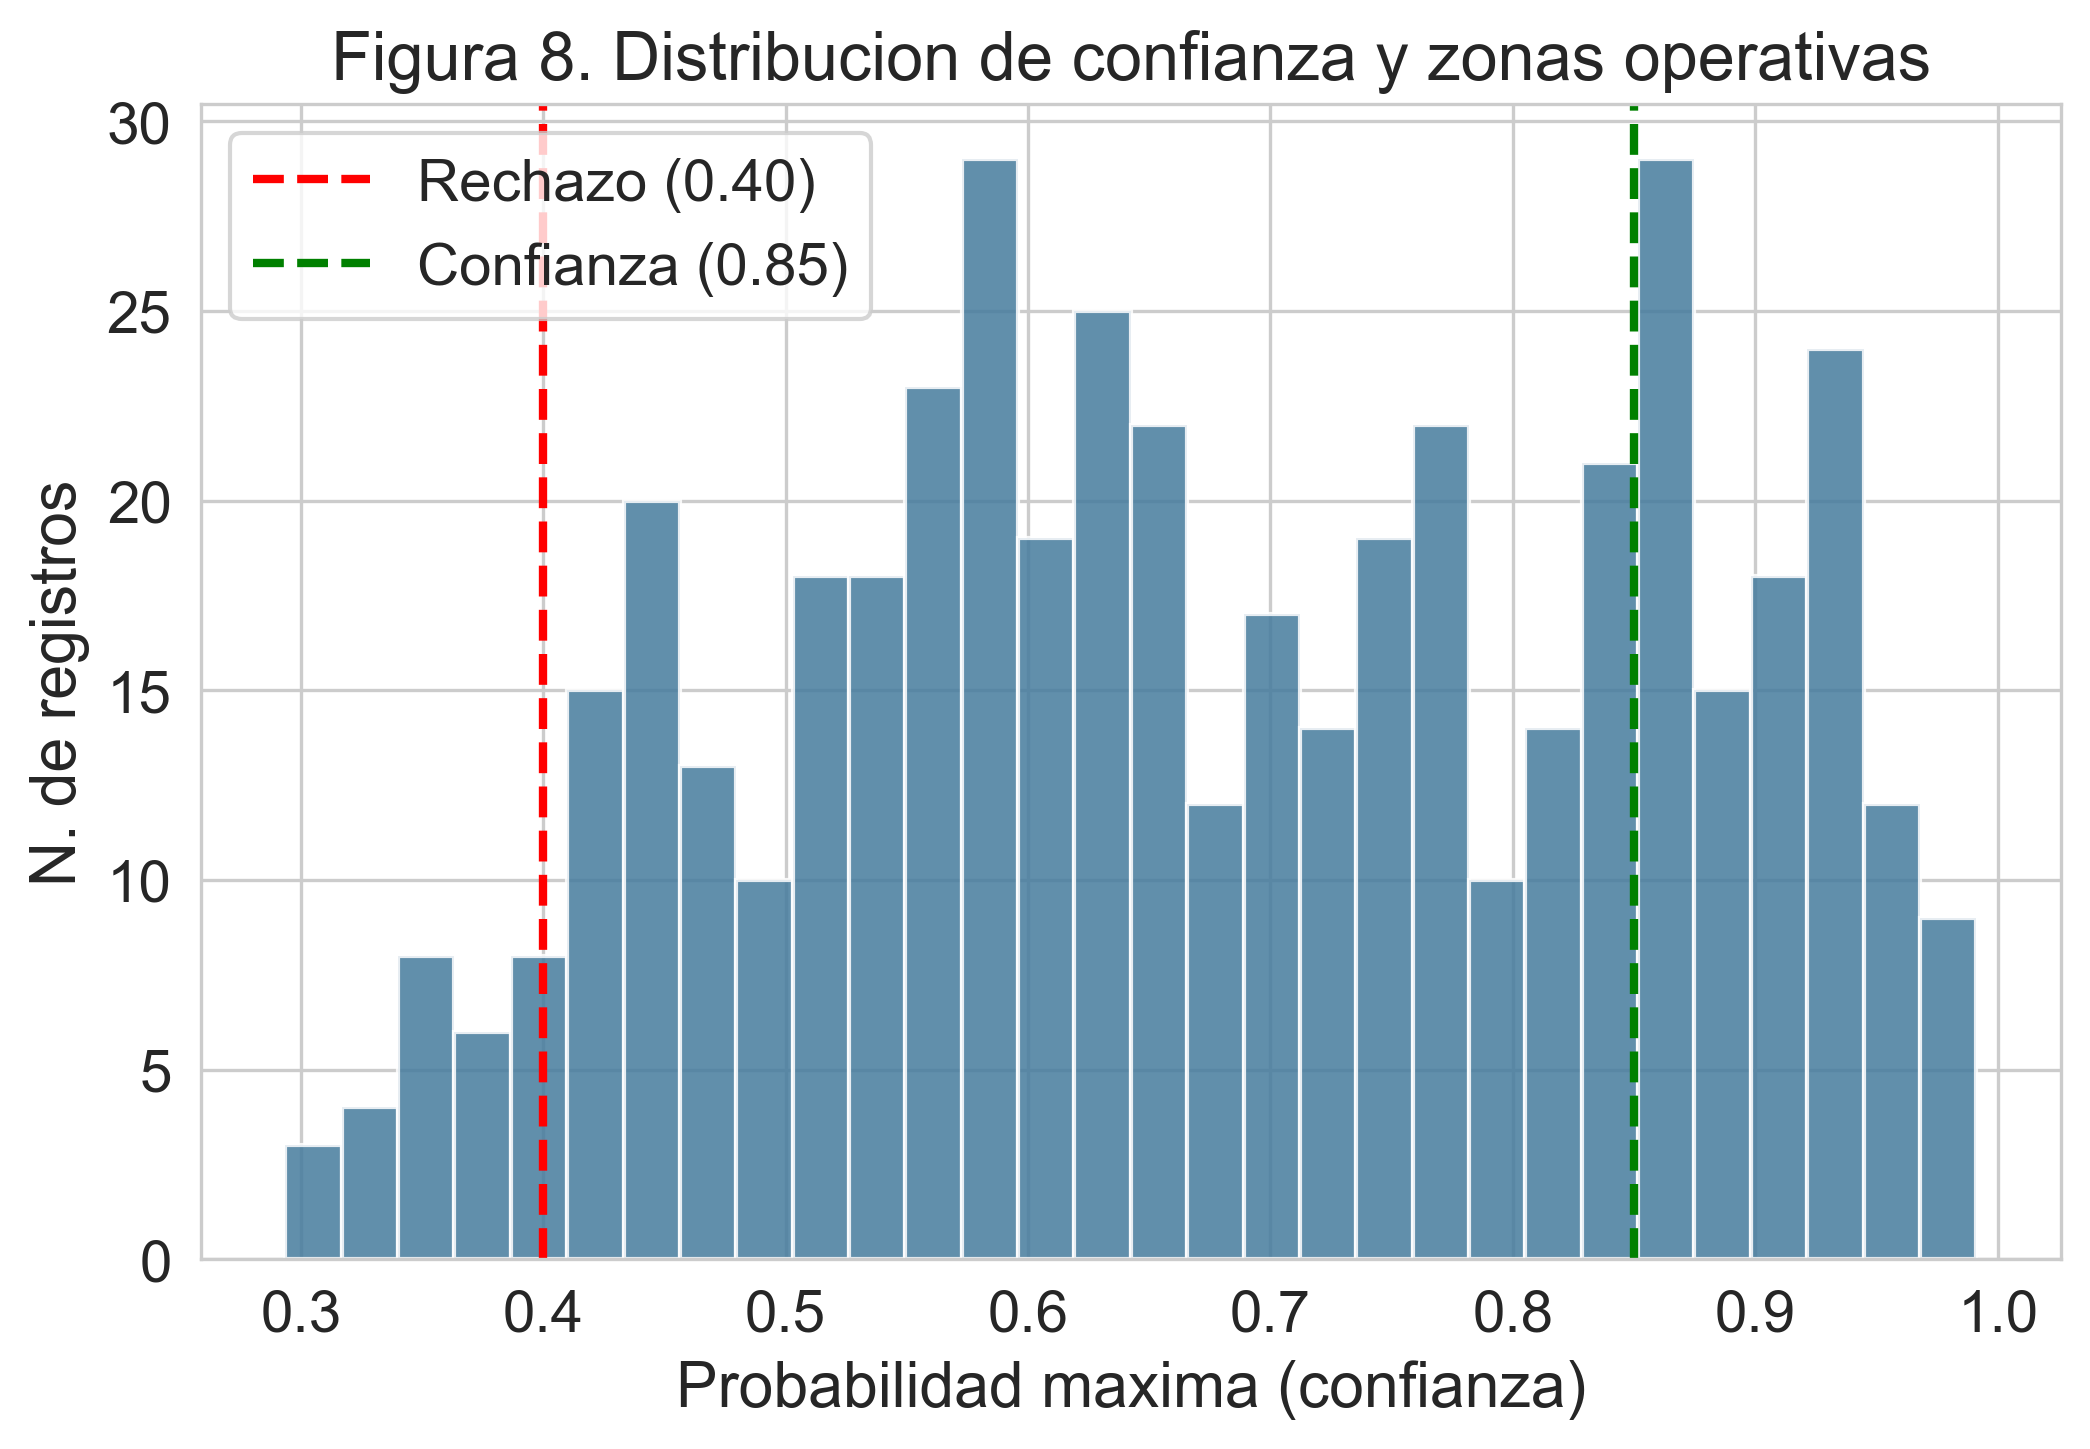
\includegraphics[width=0.6\textwidth]{figs/fig8_zonas_confianza.png}
\caption{Distribuci\'on de la probabilidad m\'axima (confianza) del modelo y zonas
operativas definidas por los umbrales 0.40 y 0.85.}
\label{fig:zonas}
\end{figure}

% ===================================================================
\section*{Referencias}
% ===================================================================
\begin{enumerate}[noitemsep,topsep=2pt]
  \item McInnes, L., Healy, J., \& Melville, J. (2018). \textit{UMAP: Uniform
  Manifold Approximation and Projection for Dimension Reduction}. arXiv:1802.03426.
  \item van der Maaten, L., \& Hinton, G. (2008). Visualizing data using t-SNE.
  \textit{Journal of Machine Learning Research}, 9, 2579--2605.
  \item Chen, T., \& Guestrin, C. (2016). XGBoost: A Scalable Tree Boosting System.
  \textit{KDD '16}.
  \item Pedregosa et al. (2011). Scikit-learn: Machine Learning in Python.
  \textit{JMLR}, 12, 2825--2830.
\end{enumerate}

% ===================================================================
\appendix
\section*{Anexo A: \textit{Contribution Statement}}
% ===================================================================
\begin{table}[H]
\centering
\caption{Matriz de coevaluaci\'on del equipo de desarrollo.}
\label{tab:coev}
\small
\begin{tabular}{p{5.5cm}cp{6cm}}
\toprule
\textbf{Nombre del Integrante} & \textbf{\% Contribuci\'on} & \textbf{Tareas encargadas} \\
\midrule
1.\quad NOMBRE 1 & XX\,\% & Tareas... \\
2.\quad NOMBRE 2 & XX\,\% & Tareas... \\
3.\quad NOMBRE 3 & XX\,\% & Tareas... \\
4.\quad NOMBRE 4 & XX\,\% & Tareas... \\
\bottomrule
\end{tabular}
\end{table}

\vspace{0.5em}
\textbf{Repositorio del proyecto:} \url{https://github.com/supermanzana-git/ml-ecoacoustic-species-classification}

\end{document}
